\documentclass{article}
\usepackage{natbib}
\usepackage{multirow}
\usepackage{booktabs}
\usepackage{changepage}
\usepackage{caption} % For caption customization
\usepackage{lineno} % For line numbers
\usepackage{graphicx} % For including graphics
% Add line numbers to the document
\usepackage{geometry}


%\usepackage{hyperref}
\usepackage[colorlinks = true, linkcolor=blue, urlcolor=blue, citecolor=blue]{hyperref}
\usepackage[nameinlink]{cleveref}
\crefname{figure}{Fig.}{Figs.}

\linespread{2} 

{\Large 
	\title{Spatio-temporal variability of zooplankton standing stock in eastern Arabian Sea inferred from ADCP backscatter measurements }}
\author{Ranjan Kumar Sahu, D. Shankar, P. Amol, S.G. Aparna,  D.V. Desai}
\date{\today}
\begin{document}
	

	\maketitle
	\linenumbers
	\section*{Abstract}
	
We use acoustic Doppler current profiler (ADCP) backscatter measurements to map
the spatio-temporal variation of zooplankton standing stock in the eastern Arabian Sea (EAS). The ADCP moorings were deployed at seven locations on the continental slope off the west coast of India; we use data from October 2017 to December 2023. The 153.3 kHz ADCP uses backscatter from sediments or organisms such as copepods, ctenophores, salps and amphipods greater than 1 cm to calculate current profile. The backscatter is obtained from echo intensity using RSSI conversion factor after doing necessary calibrations. The conversion from backscatter to biomass is based on volumetric zooplankton sampling at the respective locations. Analysis of the data over 24--120 m shows that the backscatter and zooplankton biomass decrease from the upper ocean (215 ~mg$^{-3}$ biomass contour) to the lower depths. Changes are observed in the seasonal variation of the monthly climatology of zooplankton standing stock (integral of the biomass over 24--120 m water
column) as we move to poleward along the slope in EAS. The range of variation of standing stock is lowest at Kanyakumari, followed by Okha, which lie at the southern and northern boundary of the EAS, respectively. Complementary variables are used to explain the processes leading to growth or decay of zooplankton biomass.  While annual cycle is predominant at NEAS, it decreases towards SEAS where the semi-annual cycle tends to dominate. Analysis reveals weak presence of annual cycle in zooplankton biomass and it is dominated by intraseasonal and intra-annual components. A strong intraseasonal cycle has implication on zooplankton sampling. 


	\newpage
	\section{Introduction}
	\subsection{Background}
	Zooplankton plays a vital role in food web of pelagic ecosystem by enabling the hierarchical transport of organic matter from primary producers to higher trophic levels impacting the fish population \citep{ohman2001density} and the carbon pump of the deep ocean \citep{le2016global}. They are presumably the largest migrating organisms in terms of biomass \citep{hays2003review} which occurs in diel vertical migration (DVM). Zooplankton depend not only on phytoplankton but other environmental parameters (e.g. mixed layer depth, insolation, oxygen, thermocline, nutrient availability, chlorophyll concentration and daily primary production). The biological productivity of the ocean is essentially connected with physics and chemistry \citep{subrahmanyan1959studiespart2, ryther1966primary, qasim1977biological, nair1970primary,banse1995zooplankton,mccreary2009biophysical, vijith2016consequences,amol2020modulation}. The dynamic ocean results in varying physico-chemical properties, leading to bloom and growth of plankton in favourable conditions. The changes are strongly influenced by the seasonal cycle in the North Indian Ocean (NIO; north of ~5 $^o$N of Indian Ocean). The eastern boundary of Arabian Sea contains the West India Coastal Current (\citep[WICC]{ramamirtham1965hydrography, banse1968hydrography, shetye1990hydrography,mccreary1993numerical, amol2014observed, vijith2016consequences, chaudhuri2020observed}) which reverses seasonally, flowing poleward (equatorward) during November to February (June to September). 
	
	A direct consequence of this reversal is the seasonal cycle of thermocline, oxycline and thickness of mixed Layer Depth (MLD) induced by upwelling (downwelling) favourable conditions in summer (winter) eastern Arabian Sea (EAS) facilitated further by wind speed and near-surface stratification. Further, the phytoplankton biomass and chlorophyll concentration changes with the season \citep{subrahmanyan1960studies, banse1968hydrography, levy2007basin, vijith2016consequences}. Upwelling in  summer monsoon leads to maximum chlorophyll growth in the entire EAS \citep{ banse1968hydrography, banse2000geographical, mccreary2009biophysical, hood2017biogeochemical,shi2022phytoplankton}. During winter monsoon, the convective mixing induced winter mixed layer \citep{shetye1992does, madhupratap1996mechanism,mccreary1996four, levy2007basin,  shankar2016inhibition, vijith2016consequences, keerthi2017physical,shi2022phytoplankton} results in winter chlorophyll peak in northern EAS (NEAS) while the downwelling Rossby waves modulate chlorophyll along the southern EAS (SEAS) albeit limited to coast and islands \citep{amol2020modulation}. 
	
	The zooplankton grazing peak is instantaneous with no time delay from peak phytoplankton production \citep{li2000determines,barber2001qn}, but its population growth lags \citep{rehim2012dynamical, almen2020temperature} depending on its gestation period and other limiting aspects. While some studies suggest that the peak timing of zooplankton may not change in parallel with phytoplankton blooms \citep{winder2004climatic}, others indicate that lag exists between primary production and the transfer of energy to higher trophic levels \citep{brock1992interannual, brock1991phytoplankton}. The conventional zooplankton measurements, where only few snapshot/s of the event is captured gives an incoherent or incomplete understanding in terms of spatio-temporal variation of zooplankton \citep{ramamurthy1965studies, piontkovski1995spatial, madhupratap1992zooplankton,madhupratap1996lack,wishner1998mesozooplankton,kidwai2000dd,barber2001qn,khandagale2022seasonal} as much information is revealed by later studies \citep{jyothibabu2010re, vijith2016consequences, shankar2019role, aparna2022seasonal} using high resolution data. Calibrated acoustic instruments such as acoustic Doppler current profiler (ADCP) along with relevant data can be utilised to understand small scale variability \citep{nair1999arabian, edvardsen2003assessing, smith2005mesozooplankton, smeti2015spatial, kang2024acoustic}, the complex interplay between the physico-chemical parameters and ecosystem \citep{jiang2007temporal, potiris2018acoustic, shankar2019role, aparna2022seasonal, nie2023influence}, the zooplankton migration \citep{inoue2016diel,ursella2018evidence, ursella2021diel} and their seasonal to annual variation \citep{jiang2007temporal, hobbs2021marine,liu2022seasonal, aparna2022seasonal}.
	
    The relationship between backscatter and the abundance and size of zooplankton was described by \citet{greenlaw1979acoustical} wherein it was pointed out that single frequency backscatter can be used to estimate abundance if mean zooplankton size is known. A drastic increase in study temporal and spatial variation of zooplankton biomass using  backscatter-proxy came in 1990s by introduction of high frequency echo sounders, with studies \citep{flagg1989use, wiebe1990sound, batchelder00981, greene1998three, rippeth1998diur} methodically showing acoustic backscatter estimated zooplankton biomass.
	Net sampling augmented ADCP backscatter have been used to study DVM and the spatial and temporal variability of zooplankton biomass in different marine regions, such as the Southwestern Pacific, the Lazarev Sea in Antarctica and the Corsica Channel in the north-western Mediterranean Sea \citep{cisewski2010seasonal,hamilton2013links, smeti2015spatial, guerra2019zooplankton}. The first such study to exploit the potential of ADCPs in EAS was carried out by \citet{aparna2022seasonal} (A22 from hereon) using ADCP moorings deployed on continental slopes off the Indian west coast.	In their work, they showed that the zooplankton standing stock (ZSS) in fact declines during upwelling facilitated increase in phytoplankton biomass. The unusual interaction implies the break down of existing understanding of predator-prey relationship in fundamental level of marine food chain.
	
	\subsection{Objective and scope of the manuscript}
	
	A network of ADCPs has been installed off the continental slope and shelf on the west coast of India. This ADCPs have enabled a rigorous view of intraseasonal to seasonal scale variability \citep{amol2014observed, chaudhuri2020observed} of WICC. In the recent study A22 have used ADCP moorings off  Mumbai, Goa and Kollam to explain the temporal variability of zooplankton biomass. The study showed that the zooplankton peaks (and troughs) is not only non-uniform in latitude but also heavily influenced by the oxygen minimum zone, MLD and the seasonal upwelling/downwelling conditions. Stark contrast in the phytoplankton bloom and subsequence  growth of zooplankton or the lack thereof was observed in the EAS regimes.
	
    We extend the work of A22 by presenting data from four additional moorings in the EAS, showcasing the deviations of seasonal cycle from climatology, and discussing the significant intraseasonal variability of biomass and standing stock revealed by the ADCP data. The paper is organized as follows; datasets and methods employed are described in section 2. Section 3 describes the observed climatology of zooplankton biomass and standing stock. A comparison is drawn to the results of A22. Further, the seasonal cycle of zooplankton biomass and standing stock is discussed with relation to the MLD, oxygen, temperature and circulation in determining the biomass is discussed in results section 4. Section 5 delves deeper into the intraseasonal variability with summary and conclusion in section 6.
	
	\section{Data and methods}
	The  backscatter data from ADCP and the zooplankton samples collected from the periphery of mooring is described in this section. The backscatter derived from the echo intensity of the seven ADCP mooring deployed on the continental slope off the Indian west coast is the primary data we have use in this manuscript. The moorings details are summarized in \autoref{tab:table1}. In situ biomass data from volumetric zooplankton samples are used to validate and correlate with backscatter. The chlorophyll data is used to study and draw inferences for the possible zooplankton growth seasons. In addition, we have used the monthly climatology of temperature and salinity from \citet{chatterjee2012new}. 
	
	%and the net primary productivity from MODIS (Moderate Resolution Imaging Spectroradiometer) and VIIRS (Visible Infrared Imaging Radiometer Suite) from global NPP estimates (\href{http://sites.science.oregonstate.edu/ocean.productivity}{http://sites.science.oregonstate.edu/ocean.productivity}). 
	
	\subsection{ADCP data and backscatter estimation}
    The ADCPs were deployed on the continental slope off the Indian west coast (\cref{fig:map}), off Mumbai, Goa, Kollam and Kanyakumari, and later extended to three more sites to cover the entire EAS basin from Okha (22.26$^o$N) in north to Kanyakumari (6.96 $^o$N) in south. The other two ADCPs are, 1) Jaigarh at central EAS (CEAS) to NEAS transition zone (inclined towards CEAS), 2) Udupi (primarily at SEAS regime) in the transition zone between CEAS and SEAS. The extended moorings were deployed in October 2017, though Kanyakumari had been deployed earlier too. However, only Mumbai, Goa and Kollam were part of the previous backscatter study by A22. The moorings are serviced on yearly basis usually during October--November or sometime during September--December (depending on ship availability). The ADCPs are of RD Instruments make, upward-looking and operate at 153.3 kHz. While utmost care is taken to position the instrument at  $\sim$ 200 m depth, yet for some deployments it's shallow or deeper owing to drift caused by floater buoyancy-anchor weight balance. Data was collected at hourly interval and the bin size was set to 4 m. The echoes at surface to 10\% range ($\sim$ 20 m) means the data at these depths is rendered useless and is discarded from further use.  We have followed the methodology laid down in A22 to derive the backscatter time series from ADCP echo intensity data. The gaps up to two days are filled using the grafting method of \citet{mukhopadhyay2017st} once the zooplankton biomass time series is constructed.
    
	\subsection{Zooplankton data and estimation of biomass}
	The zooplankton  samples were collected in the vicinity ($\sim$ 10 km) of ADCP mooring site twice, once prior retrieval and again post deployment of moorings so that there is overlap in the ADCP time instance and in situ zooplankton samples. The sampling is done at the mooring location during servicing cruises on board RV Sindhu Sankalp and RV Sindhu Sadhana (\autoref{tab:table2}). Multi-plankton net (MPN) (100 $\mu m$ mesh size, 0.5 $m^2$ mouth area) was used to get samples in the pre-determined depth ranges; water volume filtered was calculated by the product of sampling depth range and the mouth area of net. The depth range and timing of sample collection was different throughout the MPN hauls (refer \autoref{tab:table2}). From 2020 onward, the depth-range was standardized to the bins of 0--25, 25--50, 50--75, 75--100, 100--150 (units are in meters). The backscatter obtained earlier is averaged in vertical corresponding to the specific MPN hauls for each site. The backscatter is linear regressed with respective biomass to establish their relationship (\cref{fig:bstobm}), which has been demonstrated in numerous previous studies \citep{flagg1989use,heywood1991estimation,jiang2007temporal,aparna2022seasonal}.
	
	\subsubsection{Biomass time series and estimation of standing stock}
	
	The zooplankton biomass time series (\cref{fig:dailynmonthly}) is created from the above derived linear relationship. The standing stock is determined by taking the depth integral of biomass over the water column. To maintain the consistency of standing stock estimation, only those deployments that doesn't lack data at any depth in the entire range of 24--120 m are considered for analysis as in A22. The lack of data in the above mentioned depth range is due to deviation in positioning of ADCP sensor in the water column. A swift alteration in bathymetry along the continental slope implies that the mooring might anchor at a different depth than planned, hence a change in the predicted position of ADCP. This leads to gap in data at few mooring sites for some year. For example, for the northern-most mooring at Okha, data is not available for the entire upper 120 m depth for the second deployment. Also at Jaigarh, where the surface to $\sim$60m data (in 3rd deployment) and Kollam, where 80 m and below (in 4th deployment) is unavailable and hence discarded from standing stock estimation. There are few deployments where no or bad data was recorded e.g, at Udupi (4th deployment) and Kanyakumari (6th deployment).  	

	\subsection{Mixed-layer depth, temperature, oxygen and chlorophyll}
	As we are using a 153.3 kHz ADCP moored at $\sim$ 150 m, the top $\sim$ 10\% of data is unusable because of surface echoes. MLD in EAS is of the order $\sim$ 20 to 40 m during summer monsoon \citep{shetye1990hydrography,shankar2005hydrography,sreenivas2008monthly} especially in the SEAS \citep{shenoi2005hydrography}, but during winter the MLD in northern NEAS remains deep \citep{shankar2016inhibition}. Although it is possible to use the near-surface ADCP data after due noise correction, it is beyond the scope of present study. The temperature data is used from \citet{chatterjee2012new}, a monthly climatology having 1$^o$ spatial resolution. Monthly climatology of oxygen data is obtained from World Ocean Atlas 2013 \citep{garcia2013oxygen} which contains objectively analyzed 1$^o$ climatological fields of in situ measurements. Previous study based on ADCP data of EAS A22 have used SeaWIFS based chlorophyll data for comparison with climatology of ZSS. The SeaWIFS was at its end of service in 2010, hence we use new chlorophyll product from Global Ocean Colour, biogeochemical L3 data obtained from  \href{https://doi.org/10.48670/moi-00280}{E.U. Copernicus Marine Service Information}. The daily data is available at a spatial resolution of 4 km. 
	
	\section{Time series and climatology}
	The high and low productive biomass regime in upper and deeper depths is demarcated using a biomass contour as in A22 wherein they chose 215 mg~m$^{-3}$ as such, and it's depth is labeled as D215. However, in the present scenario we've moorings deployed at farther ends of EAS, namely Kanyakumari and Okha. The choice of biomass contour isn't abrupt; first, it is carefully chosen to accommodate the seasonal variation, as a shift to biomass contour lower than the z215 would be unviable as our data is only till 140 m depth. For example in the case of Kollam, the D215 exceeds 140 during few months of 2022 (\cref{fig:dailynmonthly}). A higher biomass contour would lead to subdued view of the seasonal cycle as in the case of Kanyakumari and Okha where 215 mg~m$^{-3}$ biomass contour is often low enough to reach $\sim$20--30 m depths (\cref{fig:dailynmonthly}), hence z175 is chosen here. Second, it allows us to link the seasonal variation of biomass to the physico-chemical properties. Climatology of zooplankton biomass and ZSS is discussed at locations northward starting from southernmost mooring site i.e, Kanyakumari. The monthly climatology of biomass and ZSS is computed for all locations having valid data in 24--140 m depth range. Time series (climatology) of biomass is discussed in the following (\autoref{sec:climatology}) section.
	
		\subsection{Time series description}
		\label{sec:timeseries}
		A preliminary analysis of the biomass time series in daily and monthly averaged scale shows that the biomass decreases with increasing depth (\cref{fig:dailynmonthly}) at all the seven locations. Rate of biomass decrease with depth, roughly defined as the difference between mean biomass at 40 m  and 104 m depth is highest off Jaigarh and Mumbai as it has higher biomass in upper ocean (\cref{fig:compfourty} c,b) and lowest off Kanyakumari. This is followed by CEAS locations Goa and Udupi (\cref{fig:compfourty} d,e). While the biomass decrease with depth is lower off Kollam from 2017 to 2020, it becomes considerably high from thereon (\cref{fig:compfourty} f). A comparatively weaker decline in zooplankton biomass with respect to depth off Okha (\cref{fig:dailynmonthly} a1,a2) at NEAS is agreeing with earlier reported data \citep{wishner1998mesozooplankton, madhupratap2001mesozooplankton, smith2005mesozooplankton,jyothibabu2010re}. The sites at SEAS, especially off Kanyakumari and 2017 to 2020 off Kollam also have weaker decrease \citep{madhupratap2001mesozooplankton, jyothibabu2010re, aparna2022seasonal}. However, the biomass decline with depth post 2020 off Kollam is high owing to a strong bloom in these years and is reflected as D215 deepening. D175 and D215 is deep throughout EAS during winter monsoon, but the occurrence of high biomass is distinct to each regime of EAS. Upper ocean shows considerably high biomass and ZSS during winter monsoon at NEAS. On the contrary at SEAS, the upper ocean shows higher biomass during summer monsoon even though the D215 and D175 is shallower during this period. 
		
		The mean, standard deviation of biomass, ZSS and chlorophyll are shown in \autoref{tab:table3}. A pattern develops from analysis of mean and standard deviation of biomass at 40 and 104 m, with comparatively lower mean biomass off Okha and Goa bifurcated by higher mean biomass off Mumbai and Jaigarh. Similarly, the lower mean biomass off Udupi and Kanyakumari is divided by higher mean biomass off Kollam. The sites with higher biomass tends to have higher variation over time e.g. Mumbai, Jaigarh and Kollam. Variation in the monthly average or seasonal cycle over time suggests significant interannual variability.
		
		\subsection{Climatology of zooplankton biomass and standing stock}
		\label{sec:climatology}
		\subsubsection{Southern EAS}
		During mid-March off Kanyakumari, the depth of 23 $^o$ C isotherm (henceforth D23) shallows along-with oxycline (marked by 2.1 ~ml~L$^{-1}$, a higher oxygen contour as it lies outside OMZ core) and a rise in biomass is observed (\cref{fig:zsschlclim} g1). The z175 is shallower from May onward to October and the zooplankton biomass is comparatively higher than rest of the year. From October z175 starts to deepen and the relatively high biomass in water column is maintained till late December. However, the deepening of D175 isn't reflected as an increase in ZSS because of low biomass in the entire water column. A gradual increase is seen in the chlorophyll biomass starting from April and the peak is attained in June (\cref{fig:zsschlclim} g2). The ZSS is increased in June, however the growth is minimal. There is almost no seasonal variation in ZSS off Kanyakumari (2.02 gm~m$^{-2}$ 3$\sigma$ of ZSS) as compared to the chlorophyll variation (1.53 mg~m$^{-3}$ 3$\sigma$ of Chl).
		
		At the nearest northern mooring site off Kollam (ZSS standard deviation, 3.75 gm~m$^{-2}$) a strong seasonal cycle is observed and the D215 is deeper for any given month. A higher biomass is present in the larger portion of water column and the D215 is at $\sim$ 110 m during Mar--May (\cref{fig:zsschlclim} f1). Starting from March, the D215 begins to shallow with progress in time till August. During this period, a sharp decrease is seen in the D23 ($\sim$ 80 m in June to September) while the oxycline (1.7~ml~L$^{-1}$ overshoots and reaches $\sim$ 40 m (\cref{fig:zsschlclim} f1). A decline (steep-rise) in ZSS (chlorophyll  biomass) is seen off Kollam and its minimum (peak) is attained in August (\cref{fig:zsschlclim} f2). The chlorophyll biomass decreases rapidly in the following months, while the ZSS increases and a maximum is seen during October. This feature was previously reported by A22, highlighting an imbalance in the interaction between zooplankton and phytoplankton.
	
		A similar feature is seen further north, off Udupi which sits at the transition zone of SEAS and CEAS, albeit with a relatively weaker zooplankton biomass. The peak of chlorophyll and minimum of ZSS occurs in September (\cref{fig:zsschlclim} e2) which is one month later than off Kollam. The 2.1 ~ml~L$^{-1}$  oxygen contour reaches to a much shallow depth of $\sim$ 20 m during July to October unlike any other location in EAS due to strong upwelling. The D215 vaguely follows D23; with the gradual shallowing from March onward reaching $\sim$ 60 m in September and a steep decline afterwards till November (\cref{fig:zsschlclim} e1).

		\subsubsection{Central EAS}
		The D215 seasonal trend off Goa in present study is similar to trend of D215 off Goa as described in A22. It is also analogous to D215 trend off Udupi since they are entirely restricted by D23 and 1.7 ml~L$^{-1}$ oxygen contour that closely follows it. Although we witness an increase in chlorophyll biomass during October, the D215 is restricted to the $\sim$ 50 m in this period  and the ZSS is at minimum  similar to off Udupi (Kollam) during September (August). The ZSS rapidly increases and reaches its maximum in January, sustained till March and then gradually declines. Unlike the previous locations, the biomass off Goa decreases rapidly below the z215 as reported earlier in A22, reaching as low as 60 mg~m$^{-3}$ at 130 m during June to September (\cref{fig:zsschlclim} d1).
	 
		The ZSS off Jaigarh is identical but stronger to that of off Goa, owing to higher biomass above z215 and the comparatively deeper D215 (\cref{fig:zsschlclim} c1). From the ZSS maximum in February (\cref{fig:zsschlclim} c2), it steadily decreases and attains a minimum in September, a rapid rise is seen in the following months. What's intriguing is a presence of strong variation in ZSS off Jaigarh (3$\sigma$ is 9.72 gm~m$^{-2}$, highest among all locations) although the seasonal variation in chlorophyll biomass (\cref{fig:zsschlclim} c2) is visibly non-existent (0.15 mg~m$^{-3}$ 3$\sigma$ of Chl) and lowest among all locations. This is an exact opposite scenario of Kanyakumari, where an insignificant seasonal variation in ZSS is seen even though the chlorophyll biomass varies strongly. 
		
		Starting from Kollam (\cref{fig:zsschlclim} f1) and moving northward to Jaigarh (\cref{fig:zsschlclim} c1), we see that the core of high zooplankton biomass gradually shifts from summer (off Kollam) to winter monsoon (off Jaigarh), with the transition of upper ocean zooplankton biomass happening along Udupi and Goa. On the contrary, chlorophyll biomass tends to have low seasonal range as we move northward from SEAS, with Jaigarh having the least seasonal variation. This shift along with winter monsoon facilitated deeper thermocline leads to an even larger impact on ZSS.
	 
		\subsubsection{Northern EAS}
		Further north off Mumbai the D215 is deeper in December to early April, resulting in a higher ZSS (\cref{fig:zsschlclim} b2). D23 follows D215 and the oxycline follows an erratic pattern, reaching depths $>$ 140 m during January to March (\cref{fig:zsschlclim} b1); when a higher biomass is observed above z215. The chlorophyll biomass shows seasonal variation albeit lower than the SEAS counterpart. The ZSS increases rapidly from its minima in October in the following month as the D215 deepens and the maximum occurs in February. The chlorophyll biomass decreases from March and a gradual decrease in ZSS is seen till July, after which the ZSS basically flattens even though the chlorophyll increases. 
	
		At the northernmost site of EAS i.e, off Okha, a noticeable feature is a much higher oxygen in upper ocean except during summer monsoon, therefore  a higher oxygen contour (3.2 ~ml~L$^{-1}$) is used for the oxycline contour. Biomass above z175 is much weaker (\cref{fig:zsschlclim} a1) leading to a relatively lower ZSS (\cref{fig:zsschlclim} a2) compared to Mumbai. The D175 shallows from February to it's minimum in August. There's two chlorophyll peak off Okha, one in February due to convective mixing induced deepening of MLD \citep{wiggert2005monsoon,levy2007basin,keerthi2017physical,shankar2016inhibition} and the other during August in summer monsoon \citep{wiggert2005monsoon,levy2007basin}. The ZSS remains flat in summer monsoon period i.e, June to September, although the chlorophyll biomass increases in this time. Afterwards, ZSS gradually increases and attains its maximum in February same as the chlorophyll biomass. ZSS sustains this maximum till March, declines rapidly in April and then gradually till July.
	 
	

	 
	\section{Seasonal cycle and variability}
	\label{sec:seasonalcyclezss}
	This section will deal with a discussion on the seasonal cycle and variability of biomass and ZSS in annual and intra-annual scale along the three regimes of EAS. 
	
	To understand the variation at a specific period, say 365-days (annual cycle) or 180-days (semi-annual cycle), wavelet analysis is carried out for biomass (\cref{fig:wave40104})  and ZSS (\cref{fig:wavess}). However, if we wish to understand the variation in a specific period band, we use Lanczos filtered zooplankton biomass. It is digital analogous to physical filters used in biology labs to filter all zooplankton within a size range. The former technique gives us an idea about variation of biomass occurring with time at all period while the later shows variation of biomass within a period band of interest. Incorrect placement of ADCP or instrument issues may lead to gaps in time series data, e.g., Okha's second deployment (2019--2020) lacked data for the top 140 meters because of deeper than intended placement depth. The gaps in time series makes it hard to analyze annual cycles in regions with limited data. Therefore, we consider locations other than Okha and Jaigarh for the 40 m biomass and ZSS in annual scale. 
		
	The biomass time series is decomposed into distinct period bands spanning days to months. Among these DVM is the simplest variation, determining zooplankton biomass at a given depth with higher (lower) biomass at night (day). On a longer time scale,  annual variability reflects changes over the course of a year often influenced by seasonal cycles like monsoons. For example, in the case of phytoplankton, upwelling favored by monsoonal winds can vary from year-to-year, thus determining the biomass for a given year uniquely. Intra-annual variability captures fluctuations that occur between seasons, shorter than a year but longer than a season, e.g., while both summer and winter monsoons are the growing season for chlorophyll at NEAS, the strength of bloom varies with season. Intraseasonal variability is about shifts occurring within a season, typically lasting weeks to months and driven by short-term environmental changes, e.g., nutrient  replenishment (depletion) in short-span due to upwelling and/or entrainment (bloom). The strength and contribution of variability components changes over time  and differs between EAS regimes. For instance, in 2019 off Kollam (\cref{fig:variability}), intraseasonal variability was dominated by it's high-frequency components (period $< \sim$30 days). An increase in biomass during the summer monsoon was due to low-frequency component of seasonal cycle, i.e., intra-annual and annual variability. However, a sharp decline in August resulted from reduced intra-annual and intraseasonal variability, even with the presence of a weakly positive annual variability. 
	
	From the linear equation correlating biomass and backscatter, the upper and lower bound of error limits equals to $\sim$ 14 mg~m$^{-3}$ (\cref{fig:bstobm}). The standard deviation incorporating 99.73 \% data i.e, $\pm$ 3 * $\sigma$ of annual variability results in its range of 40 mg~m$^{-3}$. The intra-annual variability has a range of 80 mg~m$^{-3}$. This higher range of variability compared to the error range permits us to infer information reliably. 
	
	\subsection{Annual cycle and annual variability}
	\label{sec:annualvar}
    The annual cycle of biomass off Kanyakumari (Udupi and Kollam) is weak (strong), but it varies in time. For example off Kollam, the wavelet power is stronger post 2020 (\cref{fig:wave40104} f). The biomass over 24--120 m of water column is integrated to obtain the ZSS time series. The absence (presence) of ZSS annual cycle off Kanyakumari (off Udupi) is confirmed with wavelet analysis (\cref{fig:wavess} g1). To capture the annual variability, the biomass is passed through Lanczos filter within period of 300 to 400 days (\cref{fig:annual}). The annual variability off Kanyakumari (22 mg~m$^{-3}$) is least among all mooring sites, but Kollam shows strong annual variability implying the year-to-year variation of biomass is significant.
    
    Off Goa, the annual cycle of biomass is comparatively weak contrary to the results of A22, owing to shorter time record and low biomass in the recent years as reflected in its ZSS wavelet for 2018 to early 2020 (2021 and 2022) (\cref{fig:wavess} d1) resulting in a weak (strong) annual variability (\cref{fig:intraannual}) and is also seen components of biomass variability (\cref{fig:variability}). A interesting feature is observed at the core of annual filtered biomass lying at 50 m, which seems similar to the core of annual filtered along-shore current from \citet{nethery2007zm}. This alone, however, cannot be used as evidence for causation of relation.
    
    Further north, a strong annual cycle dominates the seasonal cycle of biomass (40 m and 104 m \cref{fig:wave40104}) agreeing with A22. The annual variability is strong off Mumbai and Jaigarh with 3 $\sigma$ range of 41 and 54 mg~m$^{-3}$, respectively, which is highest among EAS regimes. Biomass variability in annual scale decreases minutely with depth off Mumbai and the three CEAS sites than off Kollam (\cref{fig:annual}) similar to the observed ocean currents \citep{chaudhuri2020observed,chaudhuri2021observed}. The annual cycle and annual variability of biomass and subsequently, ZSS increases along the slope as we go northward to Mumbai from Kanyakumari.  
    
	\subsection{Semi-annual cycle and intra-annual variability}
	\label{sec:intraannualvar}
	Along with the annual cycle we observe presence of semi-annual cycle at most locations and together they constitute the seasonal cycle. The variability at intra-annual band (\cref{fig:intraannual})  tends to be stronger compared to the annual variability. Much like the annual cycle, the semi-annual cycle and intra-annual variability is weak off Kanyakumari compared to Kollam and Udupi. However, the strong variability in intra-annual scale is restricted to upper ocean for few years off Kollam such as during 2018, 2021 and 2022. Similar to WICC variability, the intra-annual component dominates the seasonal cycle and is strong off Kollam \citep{chaudhuri2020observed}.
	
	Off Goa and Jaigarh, the semi-annual cycle tends to be strong, specifically during 2022 when a anomalous bloom is observed throughout EAS. The semi-annual cycle weakens with depth (\cref{fig:wave40104}, d) in these locations. Intra-annual component of seasonal cycle is observed off Goa, with weak (strong) variability during  2019 (2020, 2022) (\cref{fig:intraannual}, d) and is moderately strong off Jaigarh. Spread of energy among all intra-annual periods for 2022 (\cref{fig:wave40104}) off Goa, while during 2019 and 2020 the wavelet energy is only present in the semi-annual periods resulting in a overall weaker intra-annual component (\cref{fig:variability}).
	
	The intra-annual band's strength is reduced off Mumbai and Okha as compared to CEAS and SEAS. The semi-annual cycle is moderately present at 40 m (\cref{fig:wave40104}) off Mumbai which weakens at 104 m(\cref{fig:wave40104}) resulting in annual cycle dominated ZSS. Analysis reveals the presence of moderately strong semi-annual cycle off Okha only at 104 m and it's intra-annual (annual) band is similar (weaker) in magnitude as compared to Mumbai. Excluding Kanyakumari, intra-annual variability of biomass decreases poleward with higher variation seen off Kollam, Udupi and Goa similar to the ocean currents \citep{amol2014observed,chaudhuri2020observed,chaudhuri2021observed}.
	
	
	\section{Intraseasonal variability}
	\label{sec:intsnvar}
	The intraseasonal band defined as the variability occurring between periods of few days to 90 days is split into two categories; a high-frequency (period $<$ 30 days) and a low-frequency (30 $<$ period $<$ 90 days) component. The presence of significant variation in the 30-day running mean with recurring bursts are seen in the daily data and in the  wavelet analysis of biomass at 40 m and 104 m (\cref{fig:wave40104}) as bursts during few days to a week distinctive to each mooring location. Most of these bursts are occurring due to the high-frequency component of intraseasonal band of biomass. Our primary focus is in the low-frequency component of intraseasonal variability (henceforth, intraseasonal variability) i.e, within 30--90 days. The intra-seasonal component is transient in nature and its magnitude is higher than the other two low-frequency variabilities discussed in \autoref{sec:seasonalcyclezss}. With a 3*$\sigma$ range of 80 mg~m$^{-3}$ for variability in this band, we can obtain significant inferences. 
	
	Off Kanyakumari the intraseasonal variability is much strong unlike the variability in it's annual and intra-annual bands. This, along-with the wavelet at 40 and 104 m suggests that the short-term environmental changes drives the biomass off Kanyakumari which is also reflected in the ZSS (\cref{fig:wavess} g2). Off Kollam and Udupi, the intraseasonal bursts are significant but due to an equal role of intra-annual component the biomass isn't solely driven by short-term environmental changes. Strong variability in intraseasonal scale seems to occur during August to November, for example off Kanyakumari(2018, 2019 and 2020), off Kollam (2018, 2021 and 2022) and off Udupi (2018) although it can extend to mid-summer/mid-winter monsoon for few years.
	
	Off Goa, significant peaks in wavelet spectra in intraseasonal band is present in biomass (\cref{fig:wave40104}, d1, d2) and ZSS (\cref{fig:wavess},d1). During 2019, the intra-annual variability off Goa is non-existent and with the weak annual variability, a rather constant ZSS is observed (\cref{fig:wavess}, d2) and also 40 m biomass (\cref{fig:variability}). But ZSS varies briefly during September--November of 2019 as seen by the presence of spectra intraseasonal band (\cref{fig:wavess}, d1). It occurred strongly in 2018 (\cref{fig:intraseasonal}) and later in 2020 during same transition monsoon, but the absence intra-annual band in 2019 makes it easier to comprehend the contribution of intraseasonal variability. A similar feature is noted off Jaigarh albeit with a weaker magnitude.
	
	Weak presence of intraseasonal variability (\cref{fig:intraseasonal}) is also noted in the relatively smoother 30-day rolling mean ZSS off Mumbai (\cref{fig:wavess}, b2) and Okha (\cref{fig:wavess}, a2). Although spectra in the intraseasonal band is present at 40 m off Mumbai and Okha (b2, b1 of \cref{fig:wave40104}), it is almost absent at 104 m  except for a select few years. For example, during early 2021 off Mumbai, the presence of strong intraseasonal peaks in wavelet spectra of 104 m (\cref{fig:wave40104} b2) along with 40 m (\cref{fig:wave40104} b1) shows up in the ZSS spectra (\cref{fig:wavess} b1) and also in the biomass variability in intraseasonal scale (\cref{fig:intraseasonal}). It implies that the variability can be restricted to upper ocean. Off Okha, the intraseasonal variability is lowest among all EAS sites with 3*$\sigma$ range of 64 mg~m$^{-3}$ followed by Mumbai. However, Okha has weak annual and intra-annual variability unlike Mumbai leading to least predictability.
	
	The wavelet power at different depth shows peaks in low-frequency intraseasonal band across EAS. Compared to 40 m, wavelet power at 104 m suggests a decrease in its strength at respective locations most often. The intraseasonal peaks in ZSS are strong in SEAS followed by CEAS and is weak off NEAS sites. Lanczos filtered biomass shows that the intraseasonal variability is strong during August to November off all location and is coherent in many instances along much of the EAS slope as seen during 2018 (\cref{fig:intraseasonal}). The strength of intraseasonal variability of biomass is in contrast to the WICC intraseasonal band which is strong during winter monsoon at slope \citep{amol2014observed, chaudhuri2020observed} and shelf \citep{chaudhuri2021observed}. Yet the magnitude of intraseasonal variability of biomass decreases as we move poleward much like the observed intraseasonal currents. 
   

	\section{Discussion}
	
	\subsection{Summary}
	The zooplankton biomass and standing stock across different regions of EAS was examined in this article, highlighting their spatio-temporal trends in the light of physico-chemical parameters using the multi-yearlong ADCP backscatter data from 2017 to 2023. 
	
	The findings shows notable seasonal variation in zooplankton biomass and ZSS; In SEAS the higher biomass is observed during summer monsoon, while in NEAS the high biomass is observed during winter monsoon with transition of peak biomass happening gradually along CEAS regime (\autoref{sec:climatology}). Off Kollam, a unique double peak in ZSS occurs, one during May to July and another in September to November, suggesting a complex interplay between environmental drivers and zooplankton growth (\cref{fig:zsschlclim} f2). Off Kanyakumari, the seasonal variation in ZSS is non-existent even though a dramatic seasonality is seen in primary production. Climatology shows strong decline in biomass w.r.t. depth off Goa, then NEAS sites off Jaigarh, Mumbai and Okha followed by SEAS locations off Udupi, Kollam and Kanyakumari.
	
	% edit start 	
	Seasonal cycle and variability play a crucial role in regulating biomass. A strong annual cycle is observed in Northern sites like Mumbai and Jaigarh (\cref{fig:wave40104}), with biomass peaking during winter monsoon months (\cref{fig:zsschlclim}). However, the Southern and Central regions particularly off Kollam, exhibit more complex patterns. Off Kollam, the presence of a weak annual cycle and a stronger semi-annual cycle is noted along with a moderately strong biennial cycle. The semi-annual cycle is especially prominent in the Southern EAS (\autoref{sec:intraannualvar}), where it contributes significantly to the seasonal biomass changes, while northern regions is dominated by annual cycle (\autoref{sec:annualvar}). 
	
	Intraseasonal variability is found to influence zooplankton biomass significantly, especially in the summer to winter monsoon transition months (\cref{fig:intraseasonal}), while the high frequency (period $<$ $\sim$ 30 days) variability determine changes in smaller temporal scale (\cref{fig:variability}) as seen in the daily biomass record. Intraseasonal variability is higher in the Southern EAS, with the Northern regions displaying less variance. The variability in annual scale is weak, while that in intra-annual scale is often comparable to intraseasonal variability. Investigating the similarity of biomass variability with current variability within respective bands shows that signs of currents influence on biomass but establishing the connection requires further analysis.

 	\subsection{consequences of intraseasonal variability}
	However, it is evident that the high-frequency intraseasonal variability dominates the zooplankton biomass along EAS regime (\autoref{sec:intsnvar}). A strong intraseasonal component suggests huge implications on sampling, predictability and zooplankton patchiness.
 
    \subsubsection{Implication on sampling}
    The intra-seasonal component is transient and its magnitude is higher than the low frequency variabilities (\cref{fig:variability}). In NEAS for example, the SST induced fronts that lasts one to two week (\citep{sarma2018ecosystem,sarkar2019seasonal}) can make the region more productive than the surrounding ocean with an increase in integrated Chlorophyll-a (\citep{sarma2018ecosystem}). This could be be leading to the spikes in biomass that is observed in the low-period ($<$ 30 days) intraseasonal variability as seen off Mumbai Goa and Kollam (\cref{fig:variability}). Strong dependency of zooplankton biomass on the intra-seasonal variation has implication on the sampling of zooplankton using cruises. A servicing cruise along the EAS moorings takes about 12 to 15 days excluding the time to and fro from port to first/last mooring \citep{ chaudhuri2020observed, aparna2022seasonal}. However, a sampling cruise dedicated to study the spatial variation of zooplankton \citep{madhupratap1992zooplankton,smith1998seasonal,wishner1998mesozooplankton, kidwai2000dd}, say for summer monsoon may last a month or more with coarse sampling interval and hence fail to capture the actual biomass within a season for a fair spatial comparison. One such occasion is a dip in zooplankton biomass off Kollam because of intraseasonal variability during August, 2019 (\cref{fig:variability}). The resulting biomass is low even though the primary production in SEAS \citep{ashadevi20101070, jyothibabu2010re} is high and subsequent zooplankton biomass is supposed to be high. 
    
 
    \subsubsection{Zooplankton patchiness}
 	The species distribution of phytoplankton and further zooplankton in EAS is determined by intricate play based on predation, environment, competition \citep{raghukumar2003marine} and hence the forms change \citep{madhupratap1996lack,kidwai2000dd,raghukumar2003marine, smith2005mesozooplankton,khandagale2022seasonal}, with few species dominating in certain seasons. Habitat patchiness, i.e, irregular distribution of habitats and resources in the deep-sea environment \citep{eggleston1998organism,raghukumar2003marine} contributes to high biodiversity which in turn can affect ecosystem dynamics. A high intraseasonal variability in zooplankton biomass suggests that patchiness in the deep-sea environment isn't solely driven by seasonal cycles but also occurs within individual seasons. Carefully planned sampling of zooplankton with low intervals is necessary to access the zooplankton patchiness within a season. 
 	
 	\subsubsection{Predictability}
    Though EAS shows a strong seasonal cycle of current, there are notable differences between regimes of EAS. Kollam's seasonal cycle is marked by intense intraseasonal bursts making the shelf WICC at Kollam highly unpredictable \citep{chaudhuri2021observed} and the intraseasonal variation decreases equatorward. The direction of WICC at any given time of the year can be either poleward or equatorward owing to the bursts. Assuming that advection and entrainment can influence zooplankton forms and since the annual variation of biomass is much weaker, current driven intraseasonal variations of biomass in rather unpredictable manner is expected. The zooplankton biomass varies frequently and strongly within the season itself (\autoref{sec:intsnvar}). This intraseasonal variability indicates that zooplankton populations and their patches fluctuate due to short-term changes, likely responding to factors like temperature shifts, food availability, or ocean environment. So, the current and zooplankton biomass both are dominated by intraseasonal variations much more than the annual cycle. 
    
    Finding similarity in the trend of increasing (decreasing) intraseasonal (annual) variability  of biomass and currents as we go equatorward along the EAS slope is tempting, as it indicates a link between the two. In fact, the feature observed in annual filtered biomass off Goa is similar to the alongshore component (\autoref{sec:annualvar}), with the core of biomass and alongshore current lying at same depth for both. However, a rigorous study is necessary to indicate any such relationship. On similar note, the inter-annual variability of Chl-a is less in comparison to its seasonal variability \citep{shi2022phytoplankton} much like the zooplankton. Strong peaks in intraseasonal band in chlorophyll was evident in Lomb--Scargle periodogram (figure not shown), analogous to zooplankton biomass and ZSS, but lacked concrete evidence of direct correlation.
 	  
 	
	\subsection{Conclusion}
	The results presented in this paper are based on the ADCP backscatter which is suitable for creating long-term time series of zooplankton biomass in open ocean. There are however, certain limitations to this approach. While the variation in depth is captured with in situ samples from MPN, the variation in season is not adequately addressed owing to the limitation of months when ADCP servicing cruises are undertaken. The west coast cruises for ADCP servicing are planned for the monsoon transition months but may start as early as late September till December with few exceptions such as 2022 when it was carried out in March. Since the intraseasonal and intra-annual variability is almost double that of the annual one (\autoref{sec:intsnvar}), the sampling done in particular season for biomass-backscatter comparison isn't sufficient. For a better approach to capture the  seasonal variation, more in situ samples are needed from the less explored seasons. 
	
	While we are able to infer the biomass information, any information regarding the size distribution of zooplankton and their contribution to ZSS is lost. In western Arabian sea, microzooplankton dominated the grazing processes by consuming approximately 71 \% of the primary production \citep{reckermann1997-kz,marra2005jgofs,landry2009-ti}. Mesozooplankton, in turn relied on microzooplankton for about 40 \% of their food \citep{landry2009-ti,hood2024nutrient}. However, the relative grazing importance of micro and mesozooplankton fluctuated seasonally and spatially, affecting the overall impact on phytoplankton biomass in a way that aligns with the theory of grazing control or trophic cascade \citep{ripple2016-nk} in the Arabian Sea \citep{marra2005jgofs,landry2009-ti}. To understand the intricate complexities of different forms of meso- and microzooplankton and their interaction, a robust multi-frequency, size-resolving backscatter data can be utilised. However, a mono-frequency ADCP is more than enough to capture the intraseasonal variation of zooplankton that will otherwise be left inaccessible by conventional sampling means.
	
	\section{Declaration of competing interest}
	The authors declare that they have no known competing financial interests or personal
	relationships that could have appeared to influence the work reported in this paper.
	
	\section{Acknowledgments} 
	The data were collected by xxx with fund provided under xxxx. The mooring programme is supported by INCOIS (Indian National Centre for Ocean Information Sevices, Hyderabad) and CSIR. We acknowledge the contribution of mooring division and ship cell of CSIR-NIO. 
	
	Ranjan Kumar Sahu expresses his acknowledgment to the Council of Scientific and Industrial Research (CSIR) for sponsoring his fellowship. Additionally, he extends his thanks to Ashok Kankonkar for providing the essential data, Rahul Khedekar for his data processing, Roshan D'Souza for his diligent work in biological data analysis. Their contributions were invaluable to the successful completion of this research.

\linespread{1.5}	
{\footnotesize 	\bibliographystyle{plainnat} % Choose a bibliography style
	\bibliography{bs_citations} % Specify your .bib file
}	

\newpage
\newgeometry{top=1in, bottom=1in} 

\linespread{1} 	
\begin{table}[htbp]

	{\footnotesize

		\captionsetup{justification=justified,font=footnotesize,skip=0.05\baselineskip} % Adjust the spacing above and below the caption
		\caption{ADCP deployment details at the locations. The temporal resolution is 1 hour, bin size(vertical resolution) 4 m. All ADCPs are operated at 153.3 kHz. The moorings are at a water column depth of ~950--1200 m on the continental slope and are serviced on yearly basis according to ship availability. The 6th column consists of Reference echo intensity (Er) for each beam, while the 7th column contains the corresponding RSSI conversion factor \citep{deines1999backscatter}.}
		\begin{adjustwidth}{0in}{0in} 
			\begin{tabular}{ccccccc}
				
				\toprule
				\multicolumn{1}{c}{}        & \multicolumn{2}{c}{Date}                                       & \multicolumn{2}{c}{Depth}                                                              & &          \\ 
				\midrule
				\multicolumn{1}{c}{\begin{tabular}[c]{@{}c@{}} Station \\ (Position; $^o$E,$^o$N) \end{tabular}} & \multicolumn{1}{c}{Deployment} & \multicolumn{1}{c}{Recovery} & \multicolumn{1}{c}{Ocean} & \multicolumn{1}{c}{ADCP} & \multicolumn{1}{c}{Er} & \multicolumn{1}{c}{Kc} \\
				\midrule
				\multirow{4}{*}{\begin{tabular}[c]{@{}c@{}} Okha\\ (67.47, 22.26)\end{tabular}}         & 01/10/2018                      & 01/12/2019                    & 996                        & 118                       & 37                          , 37                          , 37                          , 36 &                           0.42                        , 0.44                        , 0.42                        , 0.43                        \\
				& 01/12/2019                      & 04/12/2020                    & 1166                       & 312                       & 39                          , 36                          , 38                          , 36                          & 0.42                        , 0.44                        , 0.42                        , 0.43                        \\
				& 04/12/2020                      & 08/03/2022                    & 1021                       & 144                       & 41                          , 37                          , 38                          , 37                          & 0.42                        , 0.44                        , 0.42                        , 0.43                        \\
				& 08/03/2022                      & 01/01/2023                    & 1019                       & 142                       & 37                          , 38                          , 39                          , 36                          & 0.42                        , 0.44                        , 0.42                        , 0.43                        \\
				\midrule
				\multirow{5}{*}{\begin{tabular}[c]{@{}c@{}} Mumbai \\ (69.24, 20.01)\end{tabular}}        & 09/11/2017                      & 29/09/2018                    & 1025                       & 150                       & 36                          , 34                          , 39                          , 42                          & 0.40                        , 0.40                        , 0.40                        , 0.40                        \\
				& 29/09/2018                      & 29/11/2019                    & 1122                       & 125                       & 35                          , 36                          , 39                          , 42                          & 0.40                        , 0.40                        , 0.40                        , 0.40                        \\
				& 29/11/2019                      & 02/12/2020                    & 1143                       & 164                       & 37                          , 34                          , 39                          , 43                          & 0.40                        , 0.40                        , 0.40                        , 0.40                        \\
				& 02/12/2020                      & 06/03/2022                    & 1125                       & 142                       & 36                          , 34                          , 39                          , 42                          & 0.40                        , 0.40                        , 0.40                        , 0.40                        \\
				& 07/03/2022                      & 02/01/2023                    & 1103                       & 158                       & 37                          , 34                          , 40                          , 43                          & 0.40                        , 0.40                        , 0.40                        , 0.40                        \\
				\midrule
				\multirow{5}{*}{\begin{tabular}[c]{@{}c@{}} Jaigarh \\ (71.12, 17.53)\end{tabular}}       & 27/10/2017                      & 27/09/2018                    & 1039                       & 198                       & 32                          , 35                          , 33                          , 32                          & 0.45                        , 0.45                        , 0.45                        , 0.45                        \\
				& 27/09/2018                      & 30/10/2019                    & 1032                       & 164                       & 32                          , 35                          , 33                          , 31                          & 0.45                        , 0.45                        , 0.45                        , 0.45                        \\
				& 03/11/2019                      & 30/11/2020                    & 1142                       & 264                       & 32                          , 36                          , 33                          , 32                          & 0.45                        , 0.45                        , 0.45                        , 0.45                        \\
				& 30/11/2020                      & 05/03/2022                    & 1099                       & 119                       & 33                          , 36                          , 34                          , 32                          & 0.45                        , 0.45                        , 0.45                        , 0.45                        \\
				\midrule
				\multirow{5}{*}{\begin{tabular}[c]{@{}c@{}} Goa\\ (72.74, 15.17)\end{tabular}}          & 03/10/2017                      & 25/09/2018                    & 1000                       & 174                      & 35                          , 37                          , 34                          , 35                          & 0.44                        , 0.44                        , 0.40                        , 0.41                        \\
				& 25/09/2018                      & 16/10/2019                    & 969                        & 145                       & 38                          , 36                          , 36                          , 34                          & 0.44                        , 0.44                        , 0.40                        , 0.41                        \\
				& 16/10/2019                      & 29/11/2020                    & 966                        & 143                       & 44                          , 38                          , 36                          , 43                          & 0.44                        , 0.44                        , 0.40                        , 0.41                        \\
				& 29/11/2020                      & 03/03/2022                    & 985                        & 157                       & 35                          , 40                          , 35                          , 38                          & 0.44                        , 0.44                        , 0.40                        , 0.41                        \\
				& 03/03/2022                      & 05/01/2023                    & 984                        & 159                       & 35                          , 38                          , 35                          , 34                          & 0.44                        , 0.44                        , 0.40                        , 0.41                        \\
				\midrule
				\multirow{4}{*}{\begin{tabular}[c]{@{}c@{}} Udupi \\ (74.04, 12.5)\end{tabular}}         & 05/10/2017                      & 06/10/2018                    & 1028                       & 176                       & 44                          , 46                          , 29                          , 35                          & 0.45                        , 0.45                        , 0.45                        , 0.45                        \\
				& 06/10/2018                      & 18/10/2019                    & 1027                       & 179                       & 32                          , 38                          , 30                          , 36                          & 0.45                        , 0.45                        , 0.45                        , 0.45                        \\
				& 18/10/2019                      & 11/12/2020                    & 1018                       & 168                       & 33                          , 37                          , 31                          , 38                          & 0.45                        , 0.45                        , 0.45                        , 0.45                        \\
				& 11/03/2022                      & 06/01/2023                    & 1036                       & 155                       & 31                          , 32                          , 32                          , 33                          & 0.45                        , 0.45                        , 0.45                        , 0.45                        \\
				\midrule
				\multirow{5}{*}{\begin{tabular}[c]{@{}c@{}} Kollam \\ (75.44, 9.05)\end{tabular}}        & 07/10/2017                      & 08/10/2018                    & 1174                       & 200                       & 43                          , 55                          , 45                          , 43                          & 0.49                        , 0.50                        , 0.49                        , 0.50                        \\
				& 08/10/2018                      & 20/10/2019                    & 1160                       & 123                       & 49                          , 62                          , 46                          , 46                          & 0.49                        , 0.50                        , 0.49                        , 0.50                        \\
				& 20/10/2019                      & 13/12/2020                    & 1209                       & 176                       & 52                          , 61                          , 54                          , 55                          & 0.49                        , 0.50                        , 0.49                        , 0.50                        \\
				& 13/12/2020                      & 13/03/2022                    & 1129                       & 91                        & 49                          , 51                          , 46                          , 47                          & 0.49                        , 0.50                        , 0.49                        , 0.50                        \\
				& 13/03/2022                      & 08/01/2023                    & 1149                       & 164                       & 41                          , 48                          , 43                          , 41                          & 0.49                        , 0.50                        , 0.49                        , 0.50                        \\
				\midrule
				\multirow{6}{*}{\begin{tabular}[c]{@{}c@{}} Kanyakumari \\ (77.39,6.96)\end{tabular}}   & 16/11/2016                      & 08/10/2017                    & 1096                       & 252                       & 37                          , 36                          , 37                          , 37                          & 0.42                        , 0.44                        , 0.42                        , 0.43                        \\
				& 08/10/2017                      & 10/10/2018                    & 1055                       & 181                       & 32                          , 34                          , 38                          , 35                          & 0.45                        , 0.45                        , 0.45                        , 0.45                        \\
				& 10/10/2018                      & 22/10/2019                    & 1075                       & 180                       & 36                          , 34                          , 39                          , 36                          & 0.45                        , 0.45                        , 0.45                        , 0.45                        \\
				& 22/10/2019                      & 14/12/2020                    & 1060                       & 167                       & 33                          , 35                          , 36                          , 35                          & 0.45                        , 0.45                        , 0.45                        , 0.45                        \\
				& 14/12/2020                      & 14/03/2022                    & 1184                       & 287                       & 34                          , 36                          , 36                          , 35                          & 0.45                        , 0.45                        , 0.45                        , 0.45                        \\
				\bottomrule
			\end{tabular}
		\end{adjustwidth}
		\label{tab:table1}
	}	
\end{table}
\restoregeometry

\newpage

\begin{table}[htbp]
	
	{\footnotesize
		\captionsetup{justification=justified,font=footnotesize,skip=0.05\baselineskip,width=\textwidth} % Adjust the spacing above and below the caption
		\caption{\newline Volumetric samples of zooplankton of various stations. The sampling depth range is standardised for later years for bin range of 0--25m, 25--50m, 50--75m, 75--100m, 100--150m. The abbreviations are in the following manner: Okha (O), Mumbai (M), Jaigarh (J), Goa (G), Udupi (U), Kollam (K), Kanyakumari (KK); The number tags corresponds to particular cruise of a station.}
		\begin{adjustwidth}{0in}{0in} 
			\begin{tabular}{ccccccc}
				\toprule
				Sample number & Tag & Lat($^o$N)    & Lon($^o$E)   & Date & Time (IST) & Sampling depth range (m)      \\
				\midrule
				1-3         & G1  & 15.18      & 72.79      & 25 Sep 18                 & 452        & 50–25, 100–50, 150–100        \\
				4-6         & G2  & 15.16      & 72.71      & 25 Sep 18                 & 2108       & 50–25, 100–50, 150–100        \\
				7-10        & G2  & 15.16      & 72.71      & 25 Sep 18                 & 2137       & 40–20, 60–40, 80–60, 100–80   \\
				11-14       & J1  &            &            & 26 Sep 18                 & 2000       & 40–20, 60–40, 80–60, 100–80   \\
				15-17       & J2  &            &            & 27 Sep 18                 & 2000       & 50–25, 100–50, 150–100        \\
				18-21       & J2  &            &            & 27 Sep 18                 & 2100       & 40–20, 60–40, 80–60, 100–80   \\
				22-25       & M1  & 20         & 69.19      & 28 Sep 18                 & 2135       & 40–20, 60–40, 80–60, 100–80   \\
				26-27       & M1  & 20         & 69.19      & 28 Sep 18                 & 2205       & 50–25, 100–50                 \\
				28-29       & M2  & 20.01      & 69.2       & 29 Sep 18                 & 2035       & 50–25, 100–50                 \\
				30-33       & M2  & 20.01      & 69.2       & 29 Sep 18                 & 2057       & 40–20, 60–40, 80–60, 100–80   \\
				34-37       & U1  &            &            & 5 Oct 18                  & 2000       & 40–20, 60–40, 80–60, 100–80   \\
				38-40       & U1  &            &            & 5 Oct 18                  & 2100       & 50–25, 100–50, 150–100        \\
				41-43       & U2  &            &            & 6 Oct 18                  & 2000       & 50–25, 100–50, 150–100        \\
				44-47       & U2  &            &            & 6 Oct 18                  & 2100       & 40–20, 60–40, 80–60, 100–80   \\
				48-51       & K1  & 9.06       & 75.42      & 8 Oct 18                  & 421        & 40–20, 60–40, 80–60, 100–80   \\
				52-54       & K1  & 9.06       & 75.42      & 8 Oct 18                  & 449        & 50–25, 100–50, 150–100        \\
				55-56       & K2  & 9.04       & 75.4       & 8 Oct 18                  & 2027       & 50–25, 100–50                 \\
				57-60       & K2  & 9.04       & 75.4       & 8 Oct 18                  & 2045       & 40–20, 60–40, 80–60, 100–80   \\
				\midrule
				61-64       & G2  & 15.16      & 72.74      & 16 Oct 19                 & 829        & 50–25, 75–50, 100–75, 150–100 \\
				65-67       & G3  & 15.16      & 72.74      & 16 Oct 19                 & 1812       & 50–25, 75–50, 100–75          \\
				68-70       & K2  & 9.02       & 75.42      & 20 Oct 19                 & 840        & 50–25, 75–50, 100–75          \\
				71-74       & K3  & 9.04       & 75.43      & 20 Oct 19                 & 1934       & 50–25, 75–50, 100–75, 150–100 \\
				75-78       & KK1 &            &            & 22 Oct 19                 & 742        & 50–25, 75–50, 100–75, 150–100 \\
				79-82       & KK2 &            &            & 22 Oct 19                 & 1925       & 50–25, 75–50, 100–75, 150–100 \\
				83-86         & J1  &            &            & 30 Oct 19                 & 324        & 50–25, 75–50, 100–75, 150–100 \\
				87-89         & J2  &            &            & 4 Nov 19                  & 946        & 75–50, 100–75, 150–100        \\
				90-92         & M2  & 19.98      & 69.22      & 29 Nov 19                 & 1434       & 50–25, 75–50, 100–75          \\
				93-96         & M3  & 20.01      & 69.23      & 30 Nov 19                 & 958        & 50–25, 75–50, 100–75, 150–100 \\
				97-100        & O1  & 22.24      & 67.49      & 1 Dec 19                  & 937        & 50–25, 75–50, 100–75, 150–100 \\
				101        & O2  & 22.25      & 67.46      & 1 Dec 19                  & 1957       & 150-100                       \\
				\midrule
				102-105       & G3  & 15.68      & 73.22      & 28 Nov 20                 & 930        & 50–25, 75–50, 100–75, 150–100 \\
				105-108       & G4  & 15.32      & 73.22      & 29 Nov 20                 & 1558       & 50–25, 75–50, 100–75, 150–100 \\
				108-110       & J2  & 17.85      & 71.21      & 30 Nov 20                 & 1458       & 75–50, 100–75, 150–100        \\
				111-114       & J3  & 17.91      & 71.21      & 1 Dec 20                  & 1052       & 50–25, 75–50, 100–75, 150–100 \\
				115-118       & M4  & 20.03      & 69.38      & 2 Dec 20                  & 2016       & 50–25, 75–50, 100–75, 150–100 \\
				119.00        & O2  & 22.41      & 67.8       & 4 Dec 20                  & 953        & 150-100                       \\
				120-123       & O3  & 22.41      & 67.79      & 4 Dec 20                  & 2011       & 50–25, 75–50, 100–75, 150–100 \\
				124-127       & K3  & 9.11       & 75.72      & 12 Dec 20                 & 2335       & 50–25, 75–50, 100–75, 150–100 \\
				128-131       & K4  & 9.06       & 75.74      & 13 Dec 20                 & 1507       & 50–25, 75–50, 100–75, 150–100 \\
				132-134       & KK1 & 7.62       & 77.63      & 14 Dec 20                 & 1226       & 50–25, 75–50                  \\
				135-138       & KK2 & 7.62       & 77.63      & 14 Dec 20                 & 2047       & 50–25, 75–50, 100–75, 150–100 \\
				\midrule
				139-142       & G4  & 15.32      & 73.21      & 3 Mar 22                  & 823        & 50–25, 75–50, 100–75, 150–100 \\
				143-146       & G5  & 15.68      & 73.21      & 4 Mar 22                  & 1030       & 50–25, 75–50, 100–75, 150–100 \\
				147-150       & M5  & 19.99      & 69.23      & 7 Mar 22                  & 957        & 50–25, 75–50, 100–75, 150–100 \\
				151-154       & O3  & 22.24      & 67.5       & 8 Mar 22                  & 806        & 50–25, 75–50, 100–75, 150–100 \\
				155-158       & U3  & 12.5       & 74.04      & 12 Mar 22                 & 1156       & 50–25, 75–50, 100–75, 150–100 \\
				159-160       & K4  & 9.04       & 75.42      & 13 Mar 22                 & 1027       & 50–25, 75–50, 100–75          \\
				161-164       & KK3 & 6.97       & 77.4       & 15 Mar 22                 & 1220       & 50–25, 75–50, 100–75, 150–100
				\\ 
				\bottomrule
			\end{tabular}
		\end{adjustwidth}
		\label{tab:table2}
	}
\end{table}

\newpage
\begin{table}[t]
	
	{\footnotesize
		\captionsetup{justification=justified,font=footnotesize,skip=0.05\baselineskip,width*=\columnwidth} % Adjust the spacing above and below the caption
		\caption{\newline The mean, standard deviation at 40 and 104 m of zooplankton biomass (mg~m$^{-3}$), standard deviation of ZSS (gm~m$^{-2}$, 0--140 m) and chlorophyll (mg~m$^{-3}$) at 7 mooring sites are tabulated along with the standard deviation of components of biomass variability, namely intraseasonal, intra-annual and annual.The standard deviation, 3$\sigma$ of Chl and ZSS is based on the monthly climatological data while the rest are based on the respective daily data.}
	\begin{adjustwidth}{0in}{0in} 
	\begin{tabular}{ccccccccccc}
	& \multicolumn{2}{c|}{40 m biomass} & \multicolumn{2}{c|}{104 m biomass} & \multicolumn{1}{c|}{\multirow{2}{*}{\begin{tabular}[c]{@{}c@{}}decrease with\\ depth (40m – 104m)\end{tabular}}} & \multicolumn{5}{c}{standard deviation * 3}          \\ \cline{1-5} \cline{7-11} 
	& Mean             & Std            & Mean    & \multicolumn{1}{c|}{Std} & \multicolumn{1}{c|}{}                                                                                            & Chl  & ZSS  & Intraseasonal & Intra-annual & Annual \\ \hline
	Okha        & 230.42           & 22.84          & 151.68  & 25.58                    & 78.74                                                                                                            & 0.76 & 5.8  & 64.26         & 63.78        & 22.38  \\
	Mumbai      & 272.86           & 34.95          & 182.24  & 30.34                    & 90.62                                                                                                            & 0.4  & 8.69 & 70.74         & 83.52        & 41.58  \\
	Jaigarh     & 278.45           & 36.52          & 182.96  & 48.89                    & 95.49                                                                                                            & 0.15 & 9.72 & 90.3          & 87.06        & 54.3   \\
	Goa         & 235.22           & 30.34          & 163.02  & 36.54                    & 72.2                                                                                                             & 0.45 & 6.72 & 76.38         & 83.76        & 38.58  \\
	Udupi       & 247.81           & 34.37          & 169.37  & 38.8                     & 78.43                                                                                                            & 1.65 & 6.01 & 77.22         & 100.86       & 41.64  \\
	Kollam      & 272.56           & 54.94          & 198.89  & 50.08                    & 73.67                                                                                                            & 2.05 & 3.75 & 89.94         & 95.94        & 41.82  \\
	KanyaKumari & 207.07           & 30.42          & 167.63  & 20.89                    & 39.44                                                                                                            & 1.53 & 2.02 & 71.88         & 52.62        & 21.84  \\ \hline
	\end{tabular}
	\end{adjustwidth}
    \label{tab:table3}
    }
\end{table}

\newpage
\begin{figure}[htbp]
	\centering
	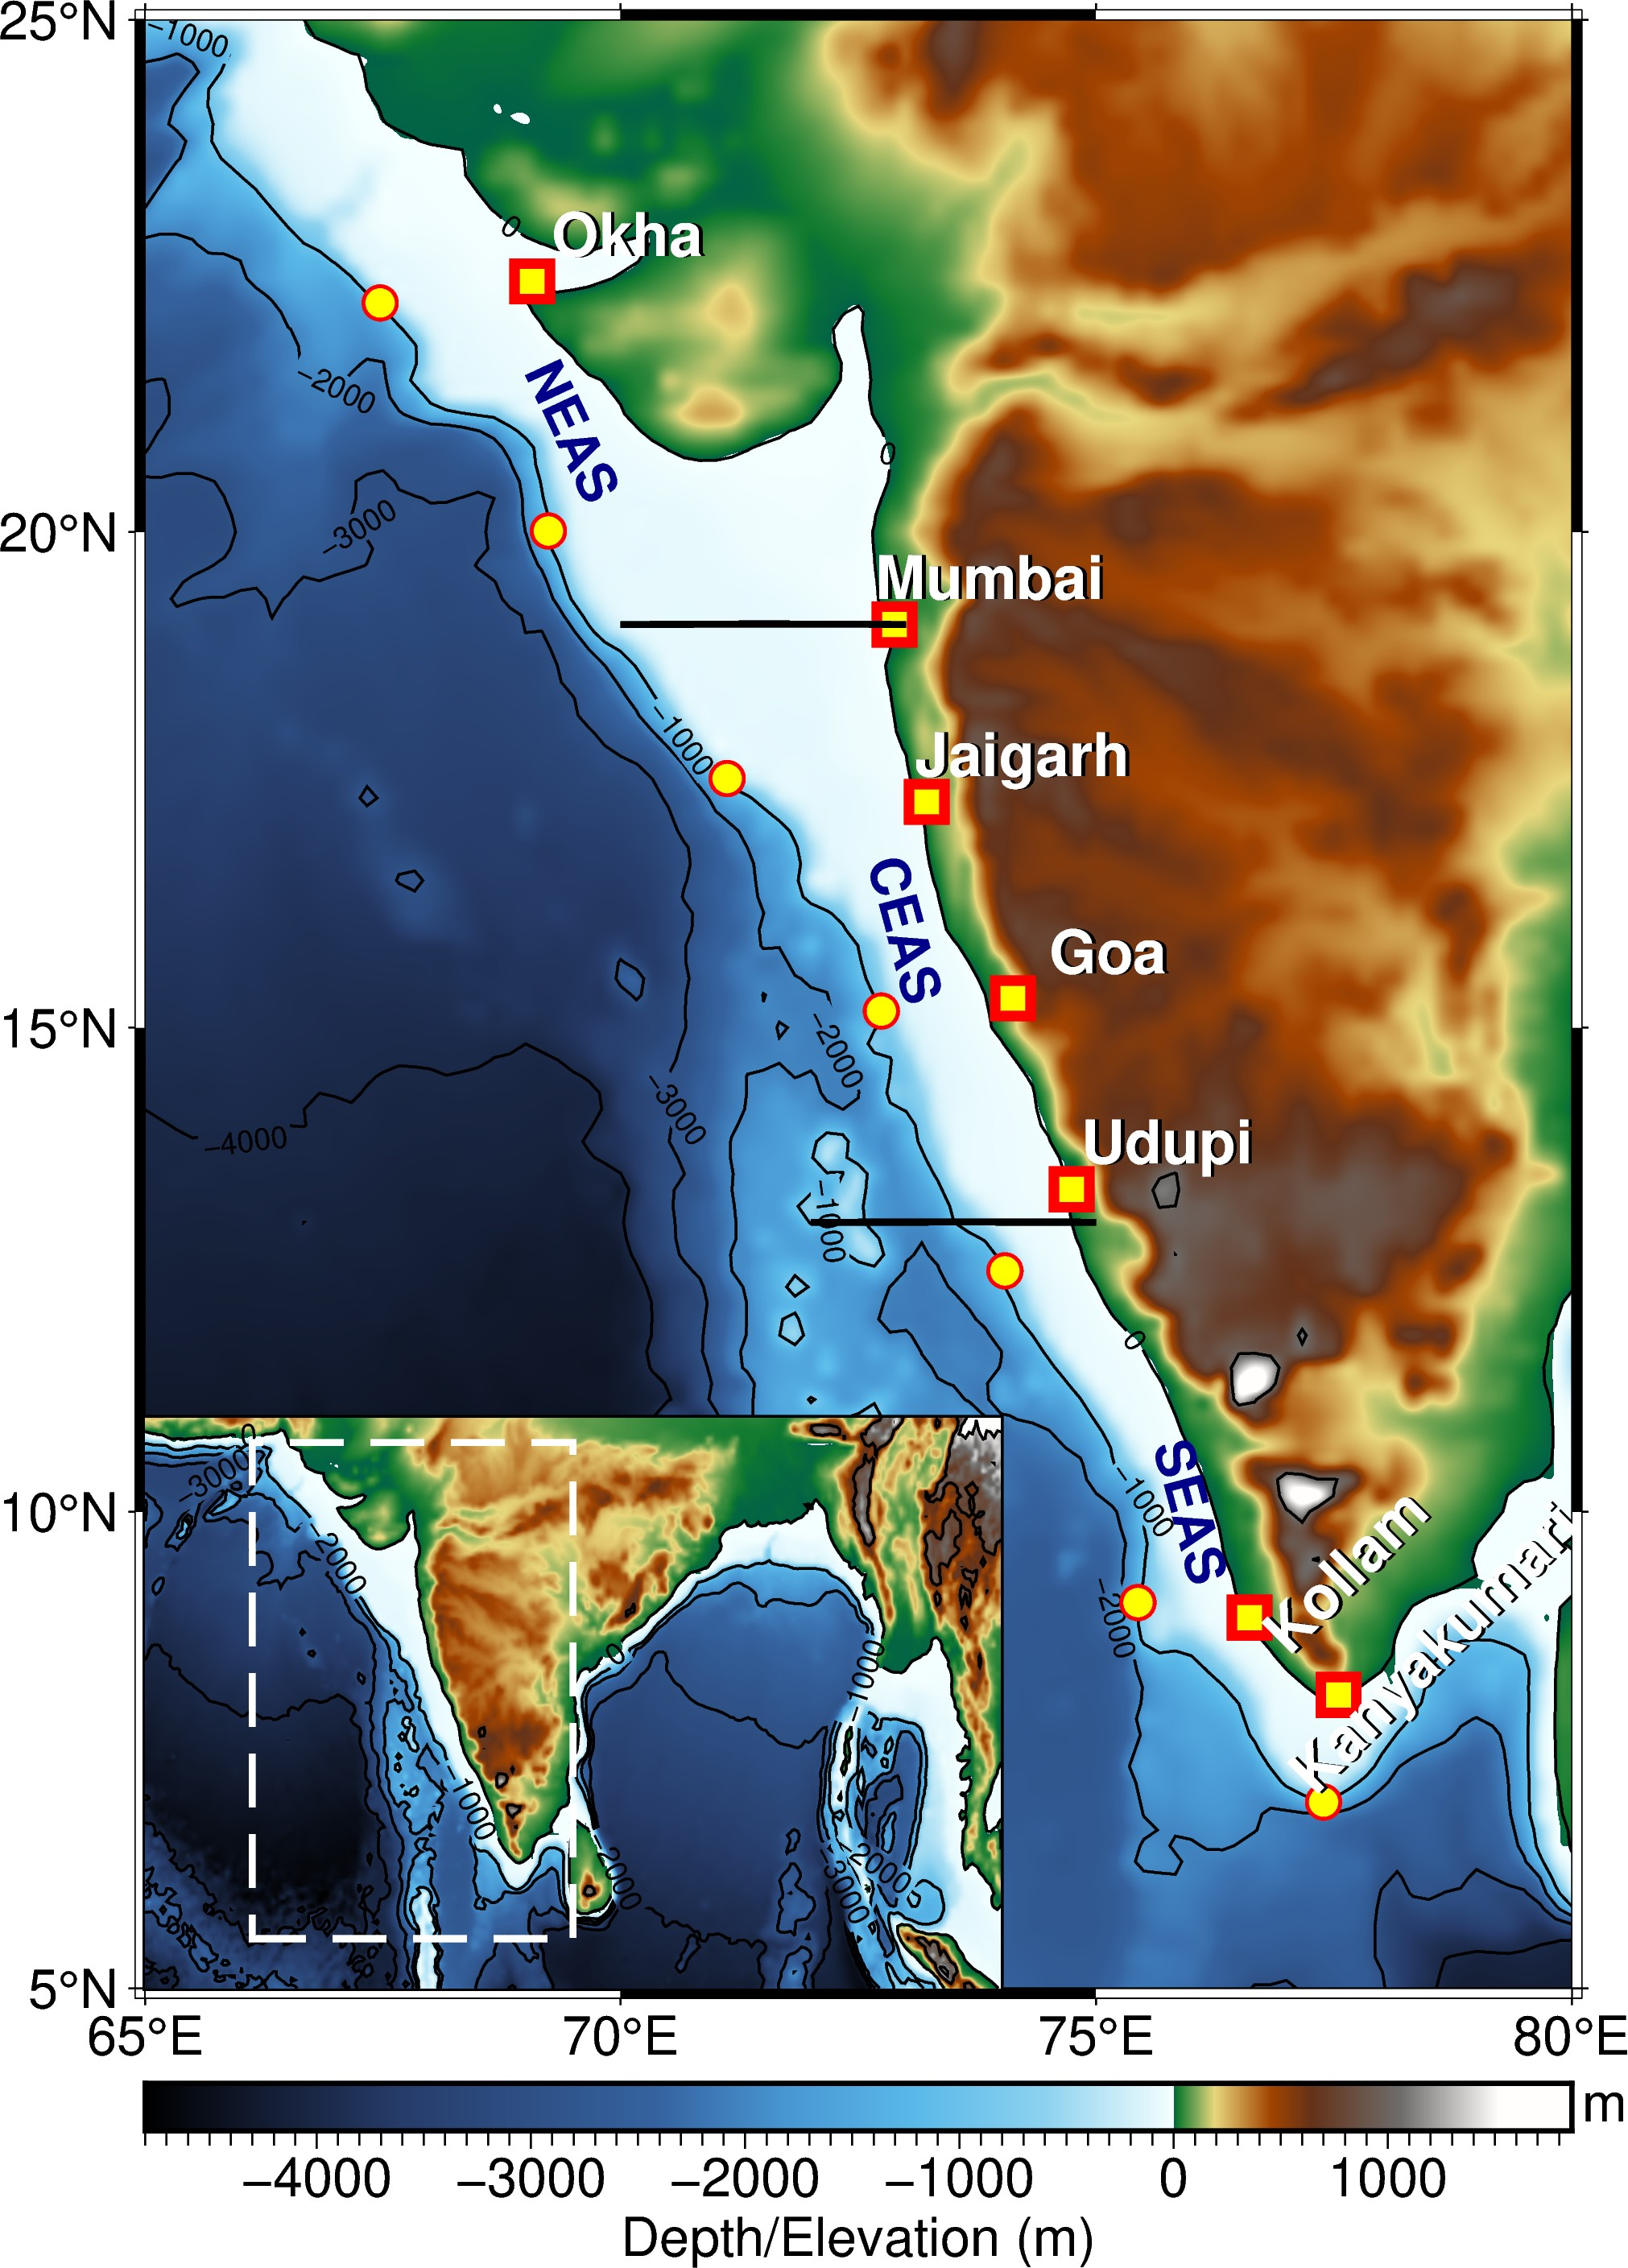
\includegraphics[width=0.6\textwidth]{/media/scilab/disk_ranjan/works/backscatter_wc/figures/adcp_moorings_new1.jpg} 
	\captionsetup{justification=justified,font=footnotesize,skip=0.05\baselineskip,width=0.8\textwidth}
	\caption{Map showing region of interest in eastern Arabian Sea. The slope moorings are
		deployed at $\sim$ 1000 m depth as shown in the bathymetry contour. Note the increase in shelf width as we go poleward along the coast. The mooring sites off Okha and Mumbai are in Northern EAS; Jaigarh and Goa in Central EAS while Kollam and Kanyakumari are at Southern EAS. Udupi is situated at the transition zone of Central and Southern EAS.}
	\label{fig:map}
\end{figure}

\newpage
\begin{figure}[htbp]
	\centering
	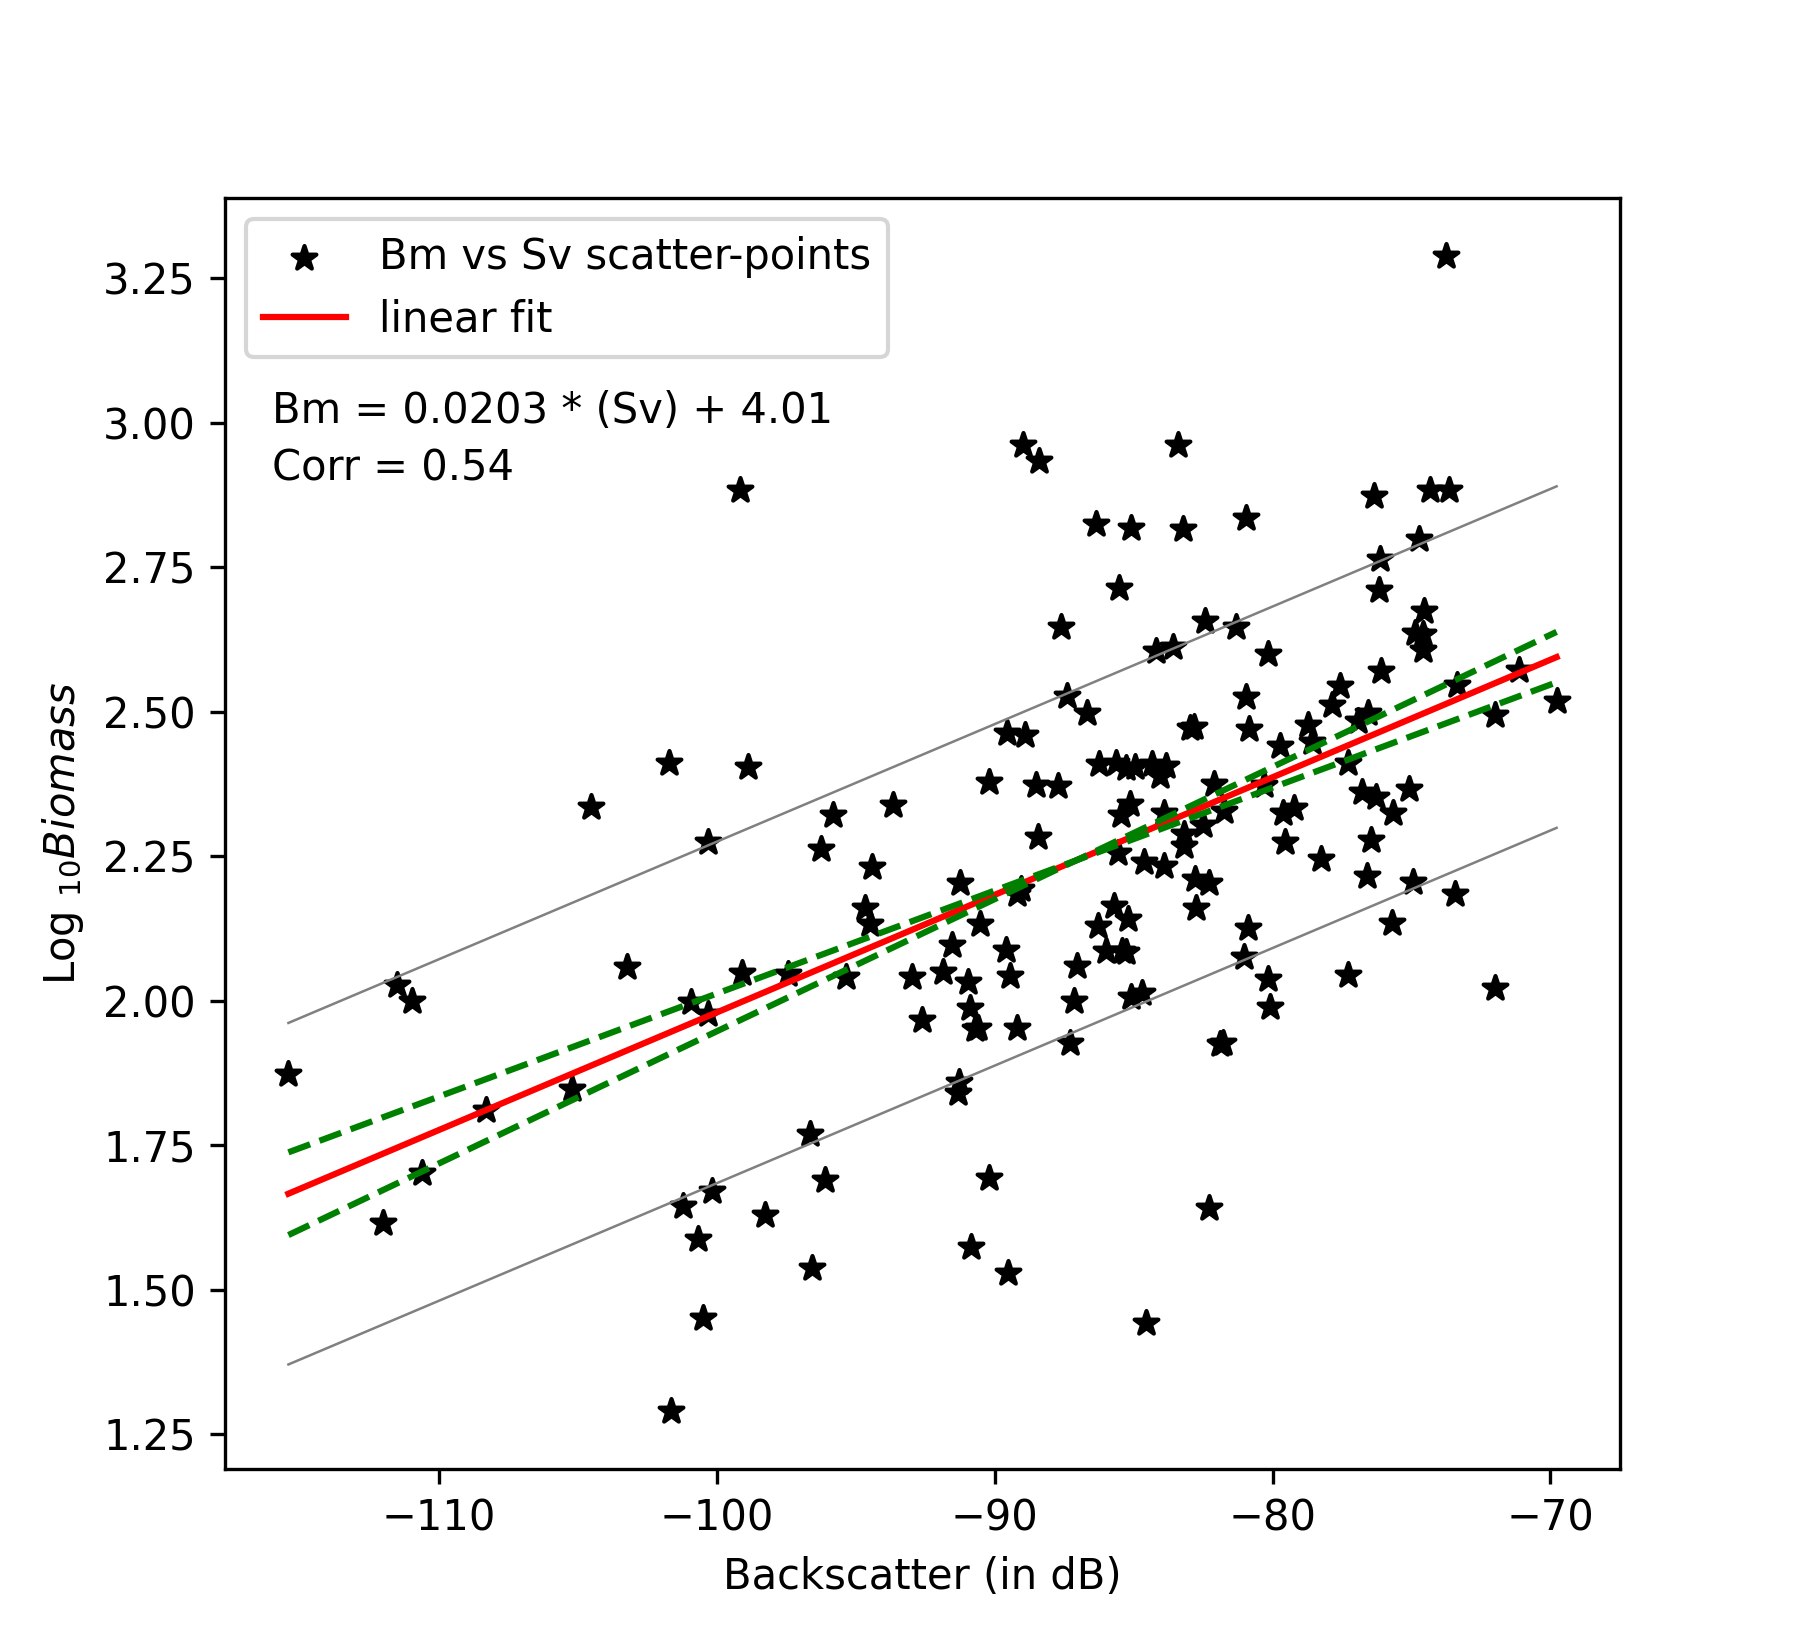
\includegraphics[width=0.5\textwidth]{/media/scilab/disk_ranjan/works/backscatter_wc/figures/backscatter_vs_biomass.png} 
	\captionsetup{justification=justified,font=footnotesize,skip=0.05\baselineskip,width=0.8\textwidth}
	\caption{The linear fit line of Biomass (log$_{10}$ scale) and backscattering strength (in dB). The linear fit line is within the error range of previous result of \citep{aparna2022seasonal} (contained 67 data points) onto which latest zooplankton volumetric sample data (159 data points) is appended. The regression equation is $y\ = (0.02 \pm\ 0.0025) \ x + (4.0144 \pm \ 0.2198) $ and correlation value of 0.54. The dashed green lines denote error range of plausible slope and intercept. From the linear equation, the upper and lower bound of error limit leads to an error bar of $\sim$  14  mg~m$^{-3}$. The first standard deviation of log$_{10}$(Biomass) is $\pm$ 0.49, which results in the backscatter range of 48.58 dB encompassing the entire backscatter range. It signifies the robustness of zooplankton biomass dependency on ADCP measured backscattering strength.}
	\label{fig:bstobm}
\end{figure}

\newpage

\begin{figure}[htbp]
	\centering
	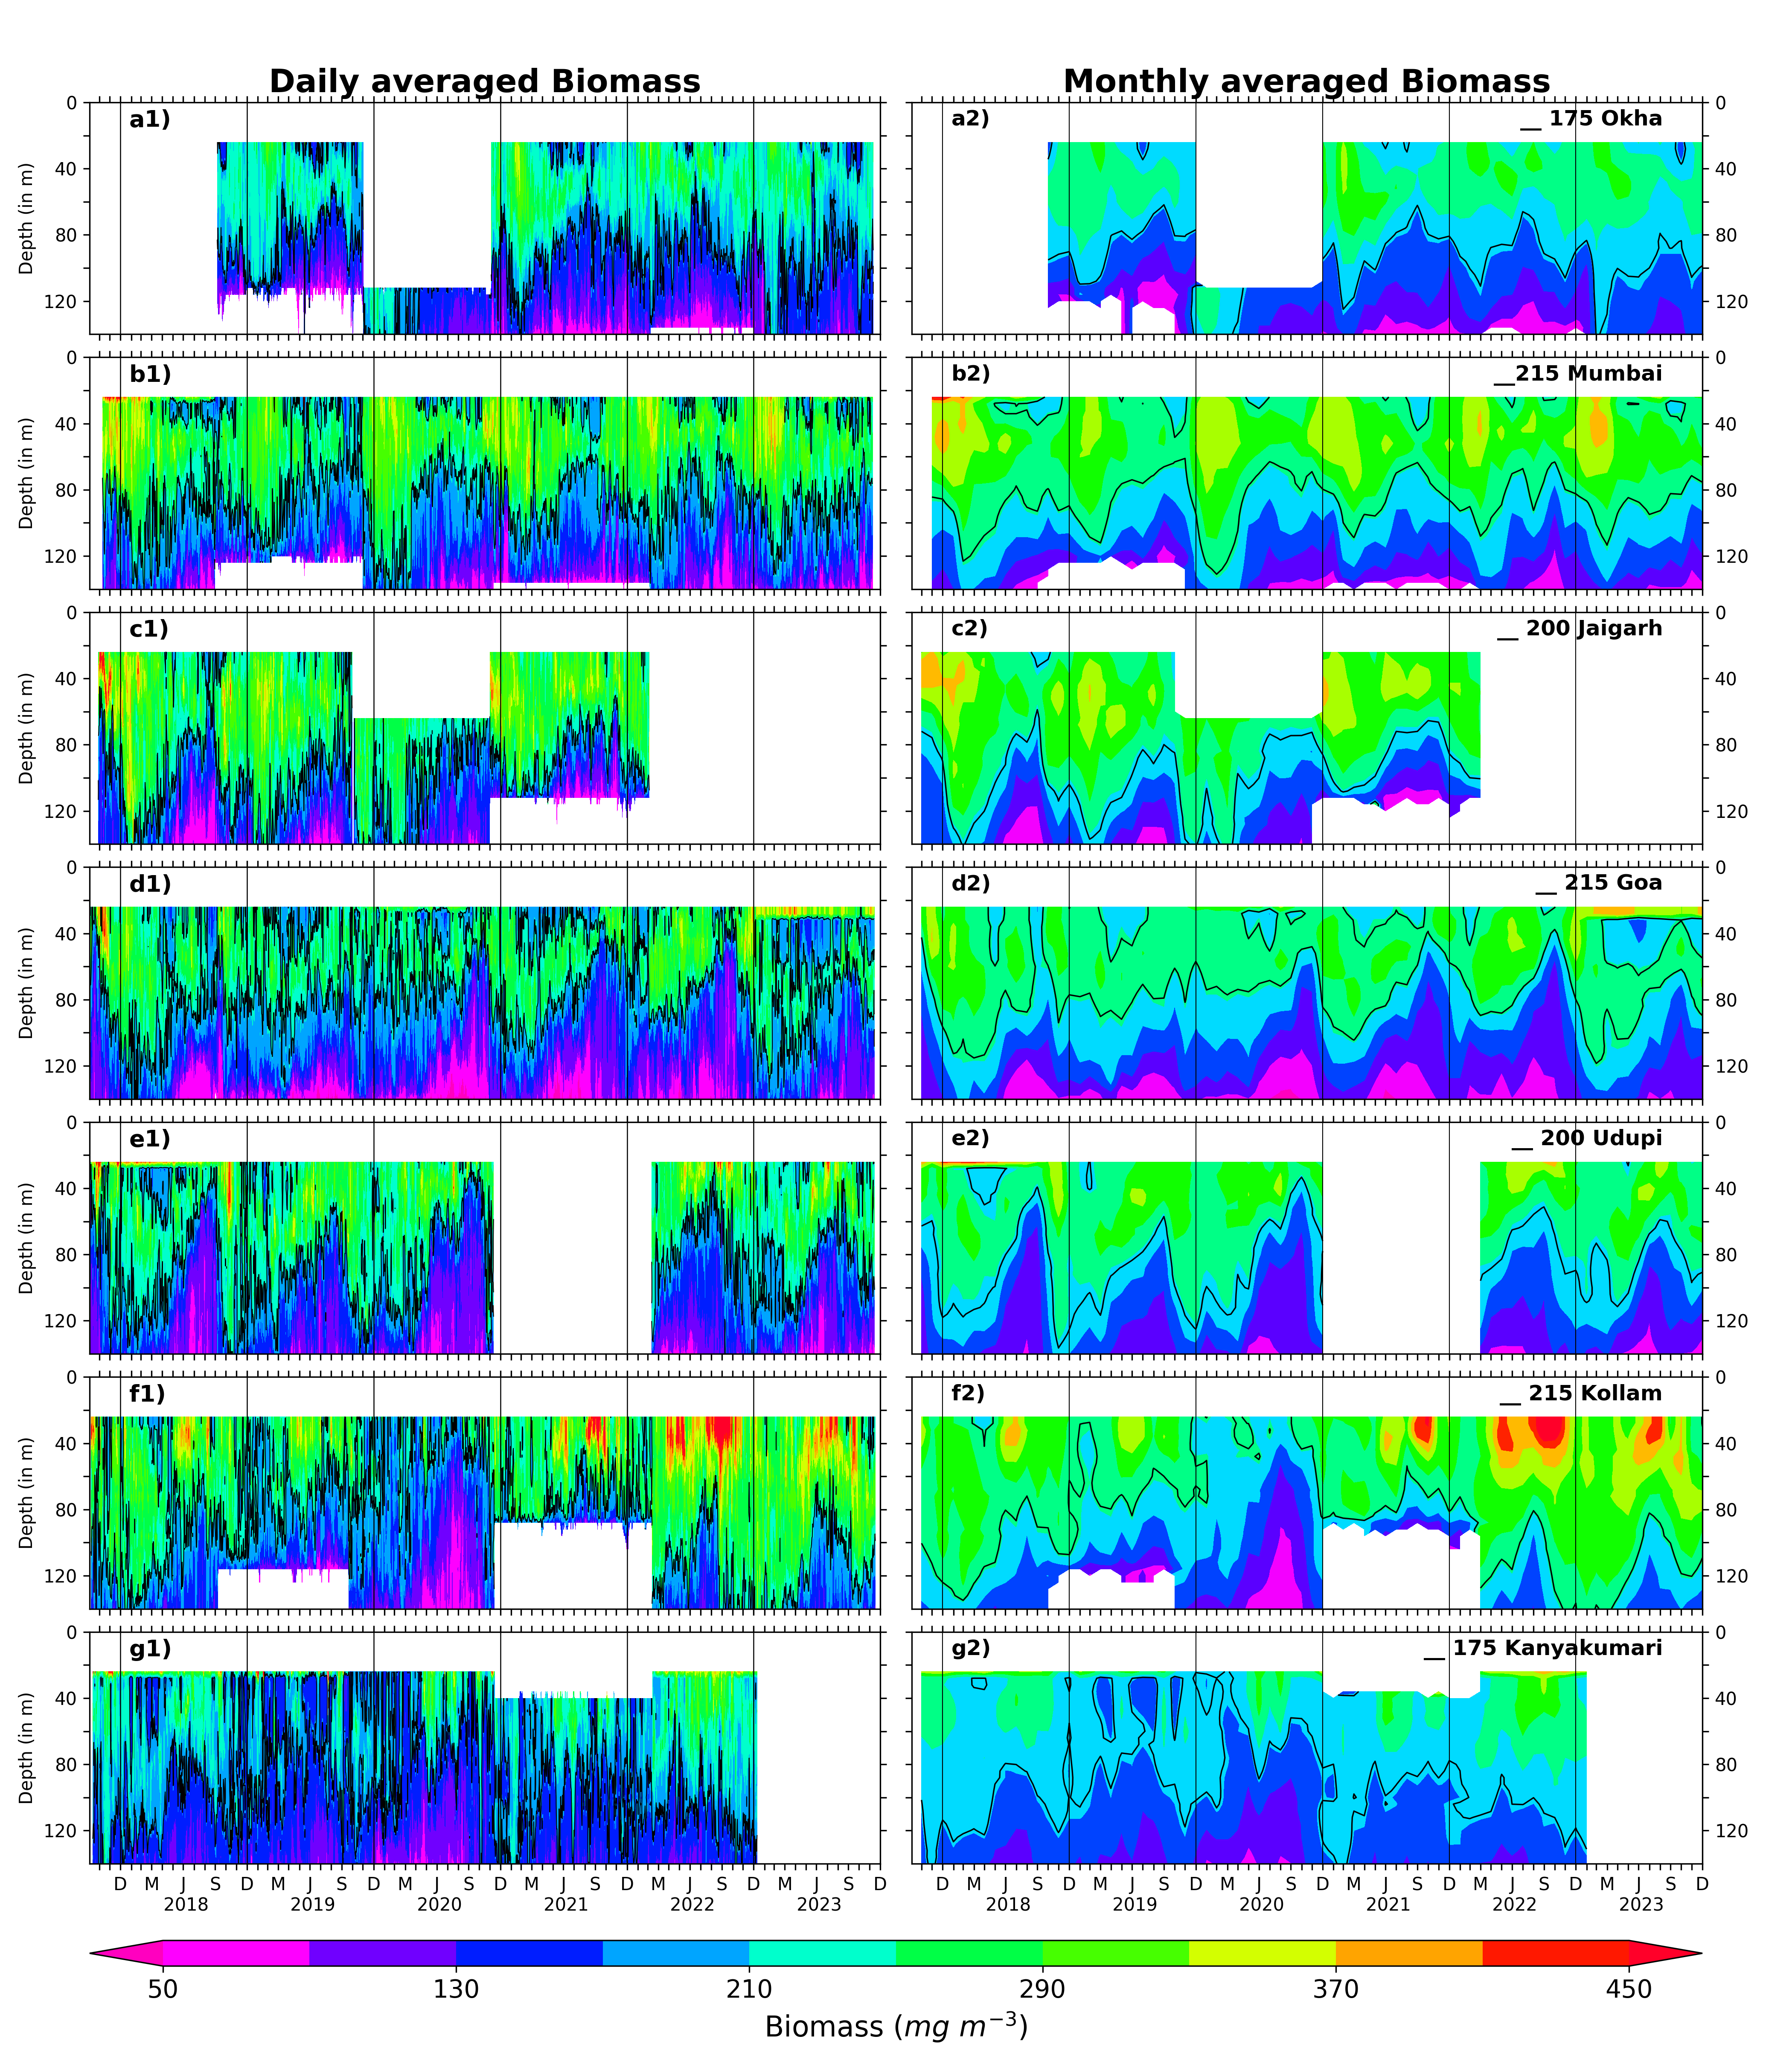
\includegraphics[width=\textwidth]{/media/scilab/disk_ranjan/works/backscatter_wc/figures/biomass_daily_monthly.png} 
	\captionsetup{justification=justified,font=footnotesize,skip=0.05\baselineskip,width=\textwidth}
	\caption{The Daily and monthly averaged biomass for EAS moorings, north (top) to south (bottom). The black contours are marking of 175 mg~m$^{-3}$ biomass for Okha and Kanyakumari; 215 mg~m$^{-3}$  for Mumbai, Goa and Kollam. The biomass contours are distinct and different based on the physico-chemical parameters and the one that best explains seasonality at respective location.  The top 10 \% of data is discarded due to echo noise. The dashed line at 22 m marks the top-depth of first bin i.e, 24 m.}
	\label{fig:dailynmonthly}
\end{figure}

\begin{figure}[htbp]
	\centering
	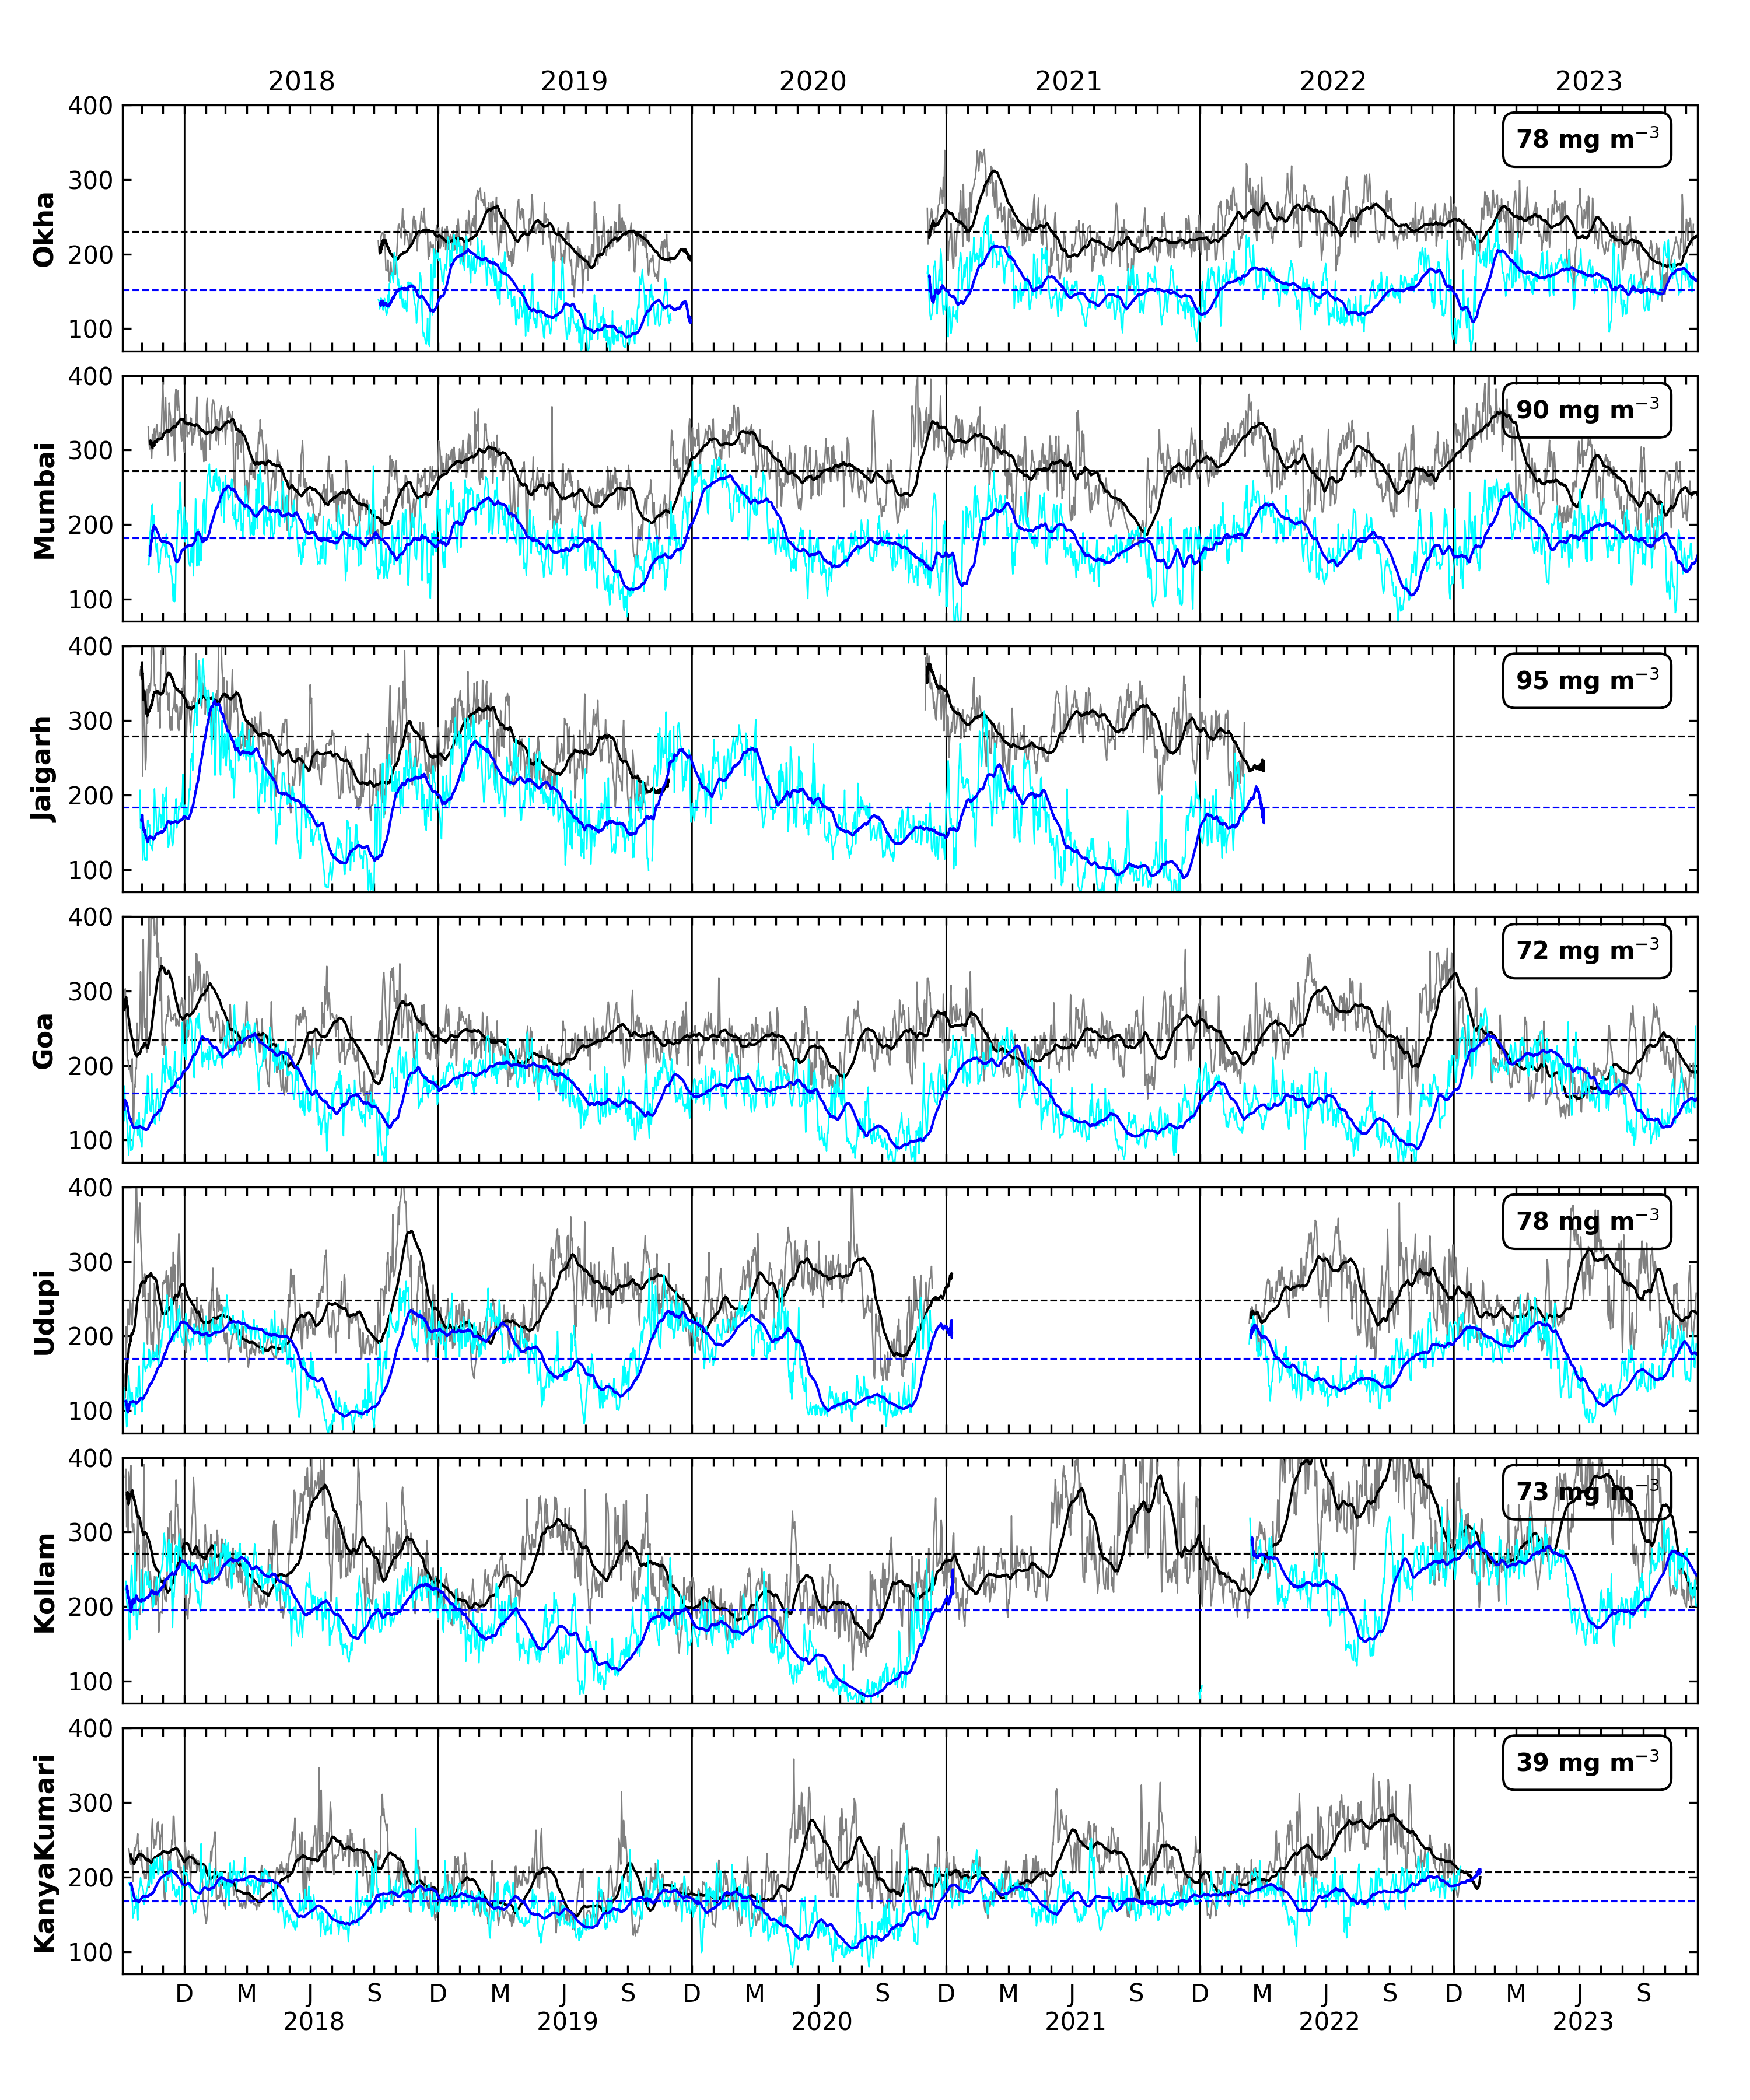
\includegraphics[width=\textwidth]{/media/scilab/disk_ranjan/works/backscatter_wc/figures/biomass_40m_104m.png} 
	\captionsetup{justification=justified,font=footnotesize,skip=0.05\baselineskip,width=\textwidth}
	\caption{The daily biomass at depth of 40 m and 104 m for all locations shown by grey and cyan curves. The black and blue lines shows the 30 day rolling averaged biomass at 40 and 104 m, respectively. Notice the bursts seen in the daily data ranging from few days to weeks.}
	\label{fig:compfourty}
\end{figure}


\begin{figure}[htbp]
	\centering
	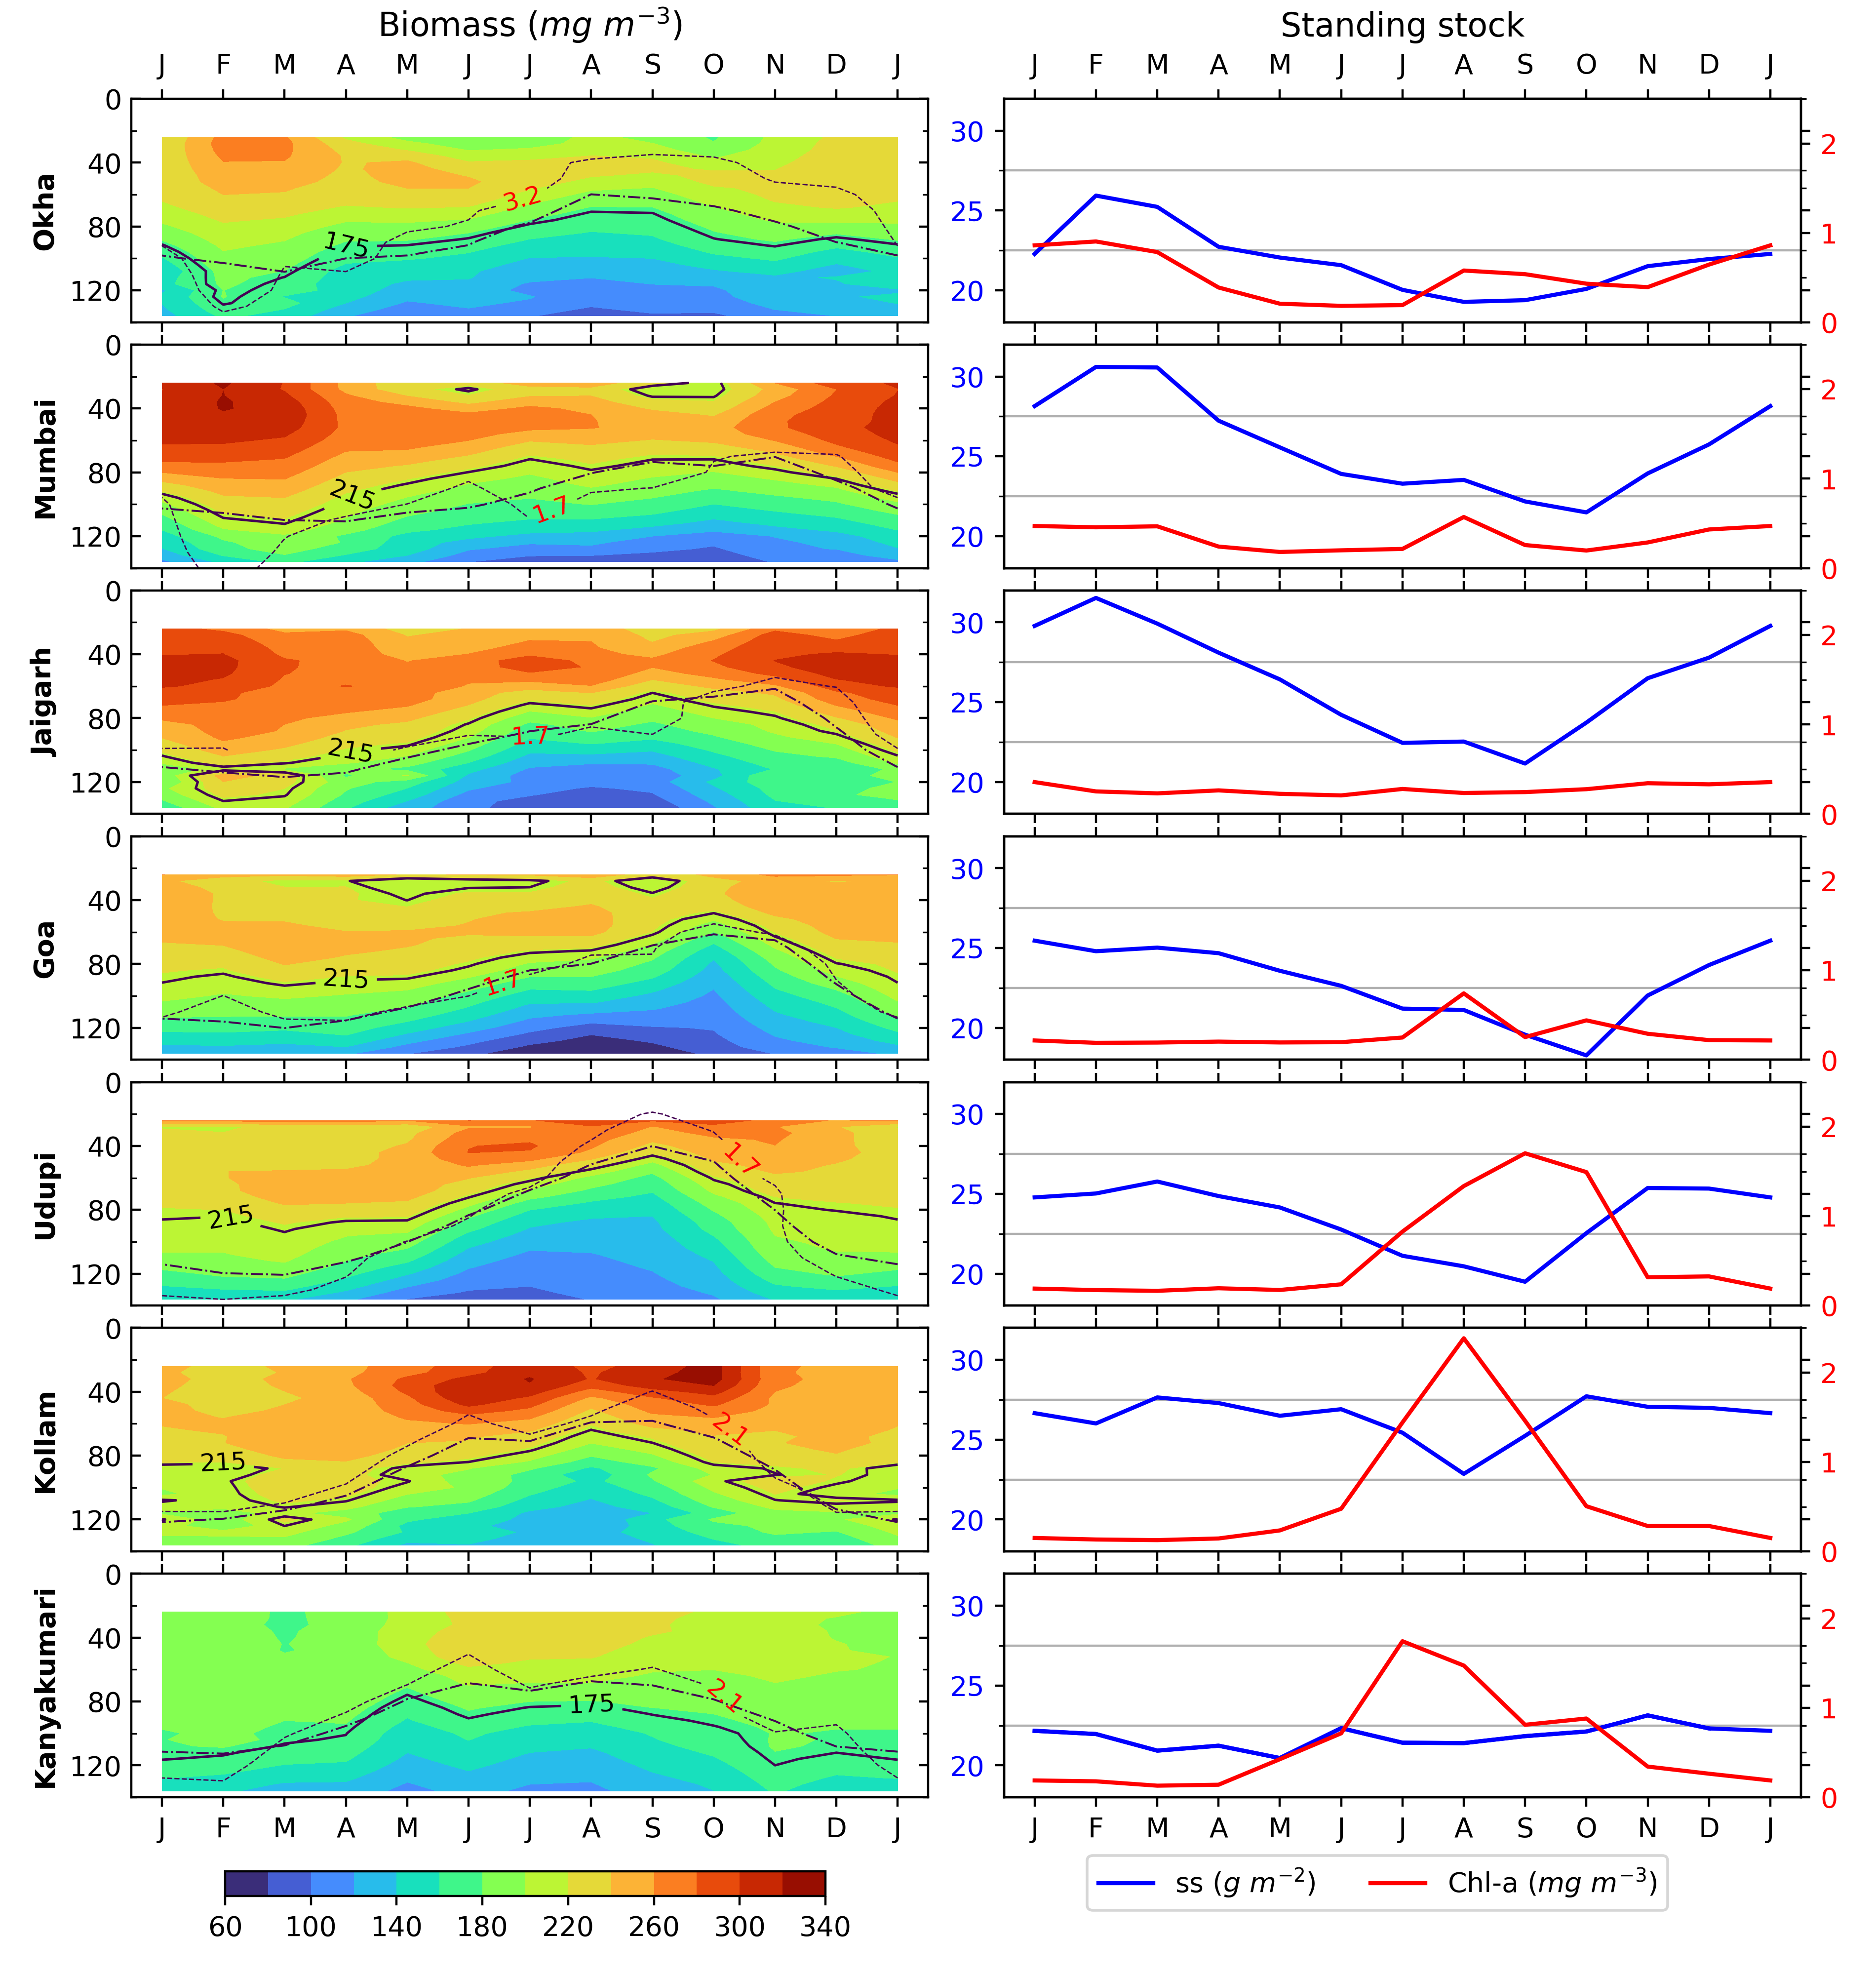
\includegraphics[width=\textwidth]{/media/scilab/disk_ranjan/works/backscatter_wc/figures/climatology_biomass_ss_chl.png} 
	\captionsetup{justification=justified,font=footnotesize,skip=0.05\baselineskip,width=\textwidth}
	\caption{Monthly climatology of zooplankton biomass is shown in left panels for 7 locations, (top to bottom is southward). The D175 and D215 are shown in solid lines; dashed line represents the depth of 23 C isotherm; oxygen contours are shown in dotted lines and labeled for each mooring. The right set of panel plots is showing ZSS (24--140 biomass integral) and chlorophyll climatology for corresponding locations.}
	\label{fig:zsschlclim}
\end{figure}



\begin{figure}[htbp]
	\centering
	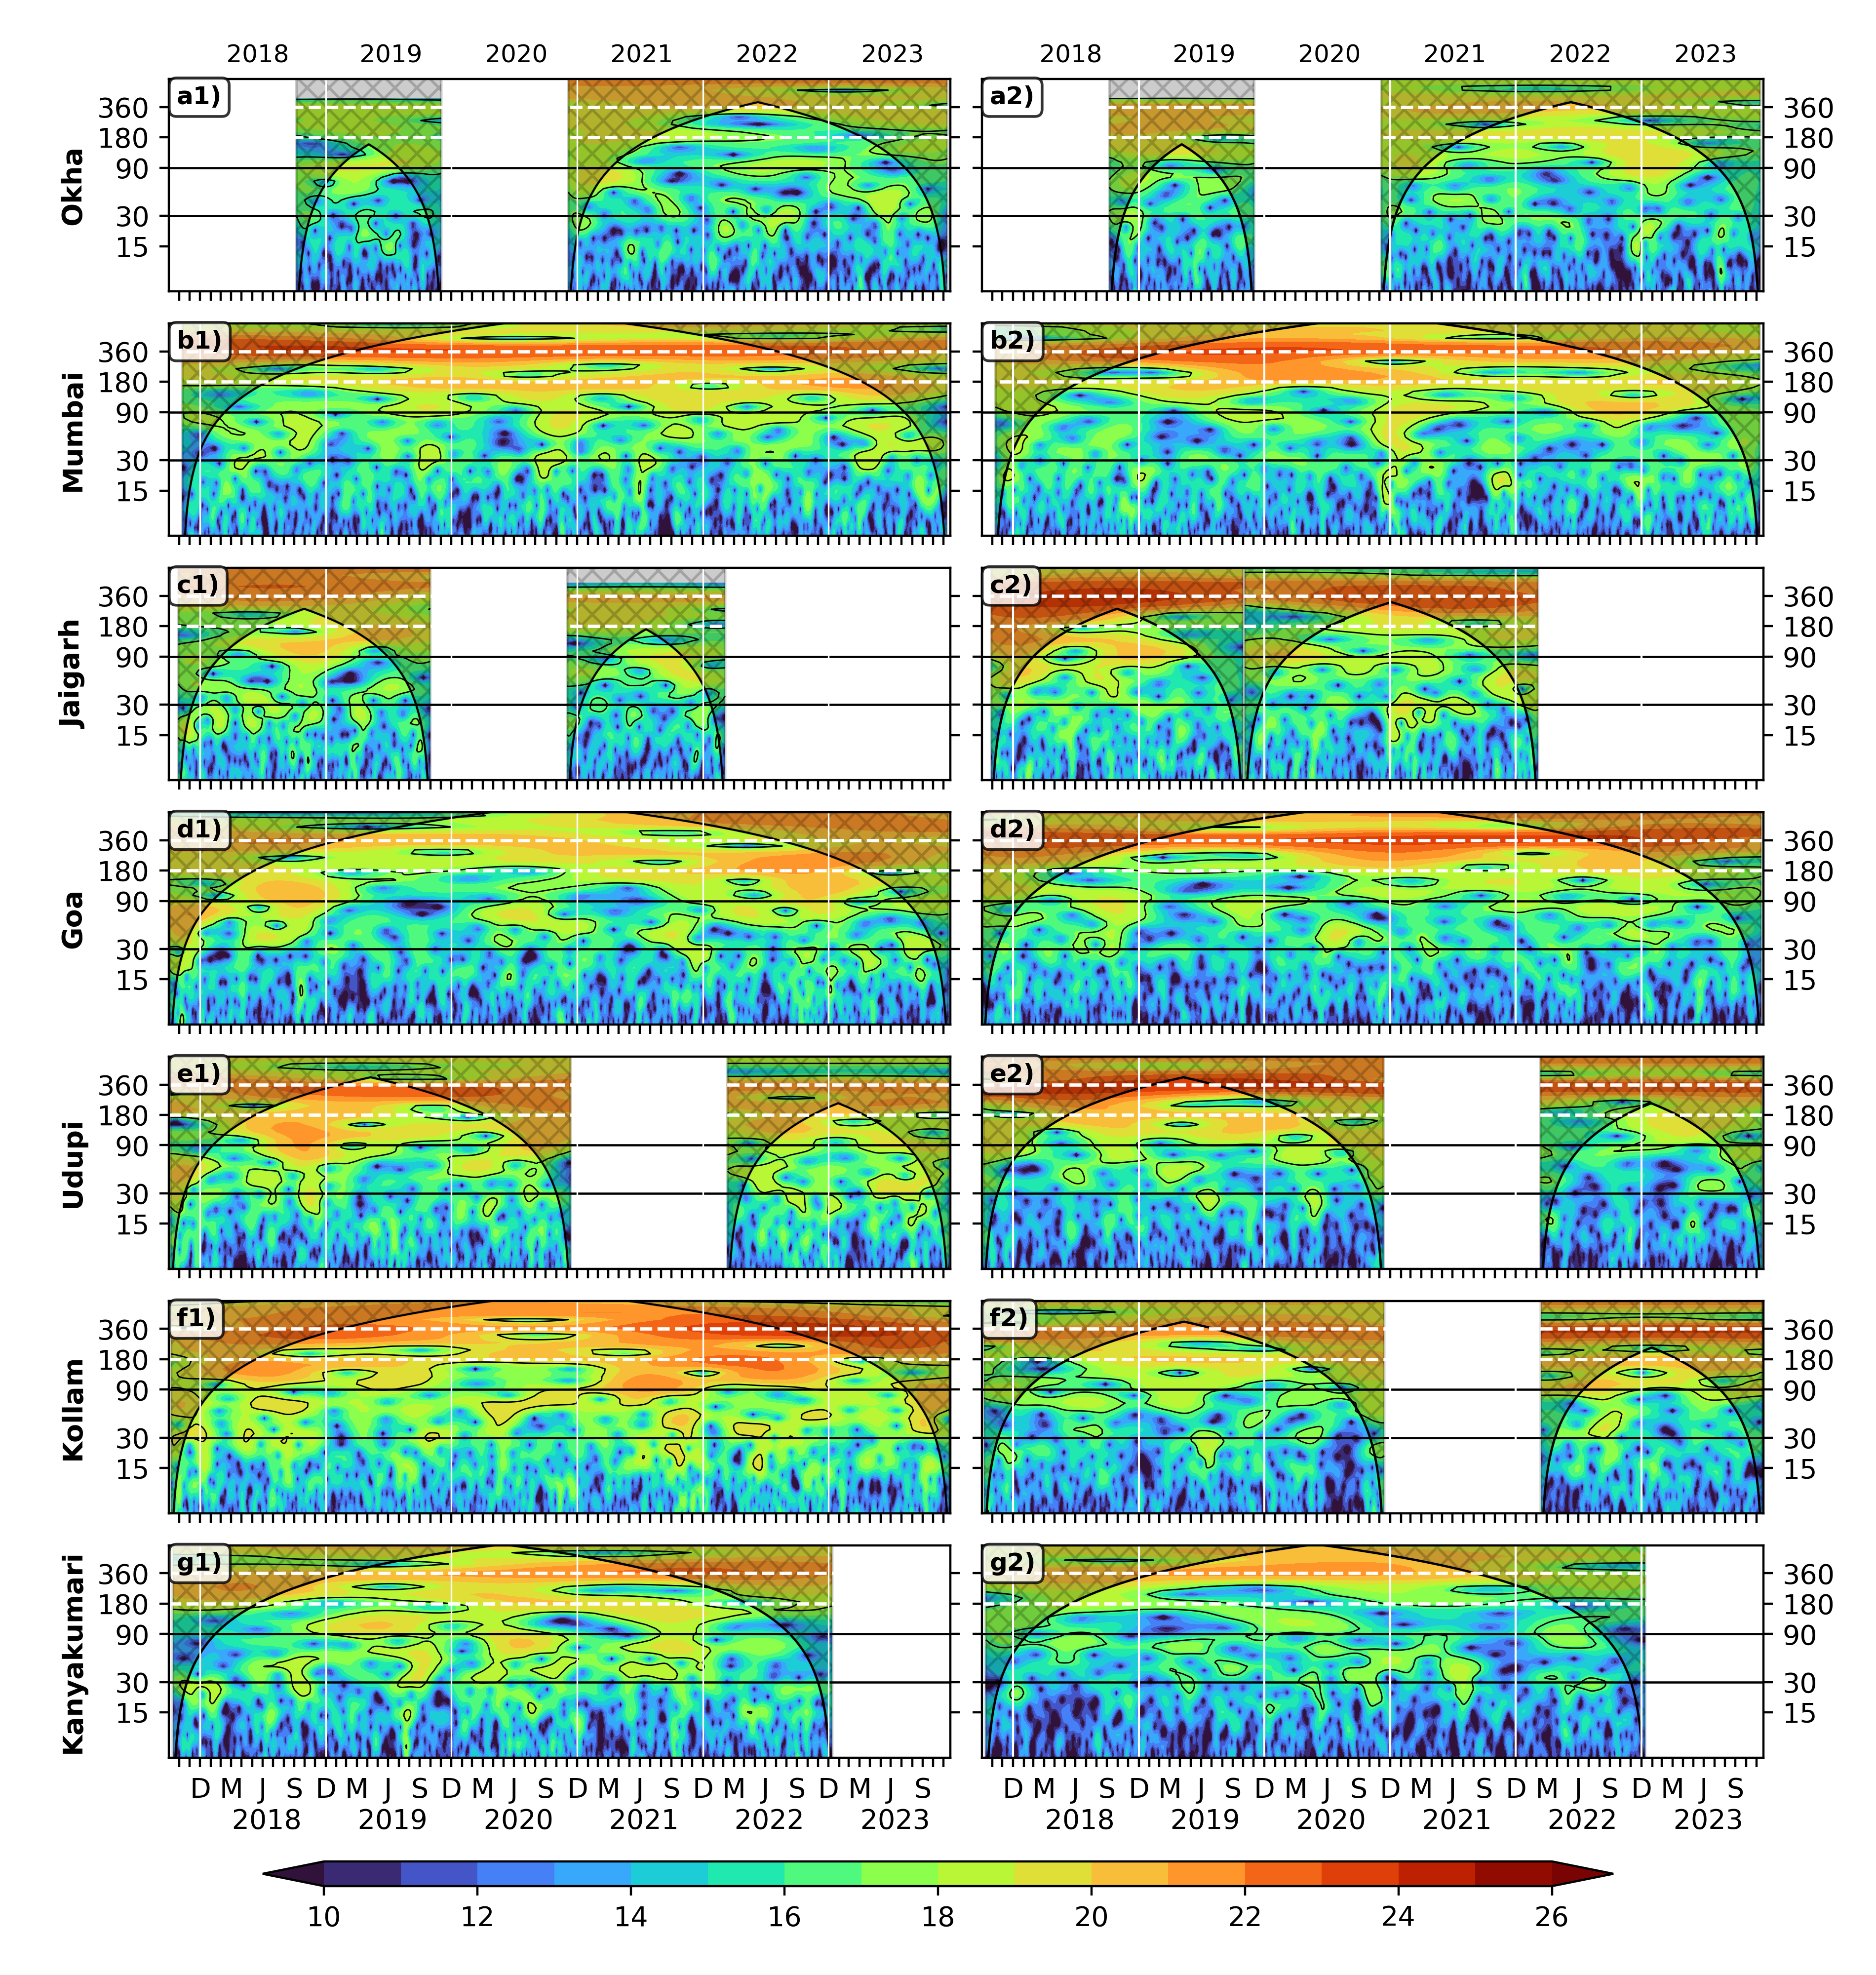
\includegraphics[width=\textwidth]{/media/scilab/disk_ranjan/works/backscatter_wc/figures/west_coast_wavelet_40m_104m.png} 
	\captionsetup{justification=justified,font=footnotesize,skip=0.05\baselineskip,width=\textwidth}
	\caption{Wavelet power spectra (Morlet) of the 40 m (left panel) and 104 m (right panel) zooplankton biomass plotted against time as abscissa and period in days as ordinate. The wavelet power is in log$_2$ scale, the 95 \% significance is marked in black contours; the cross-shaded region falls under cone of influence. Vertical white lines separates years.}
	\label{fig:wave40104}
\end{figure}


\begin{figure}[htbp]
	\centering
	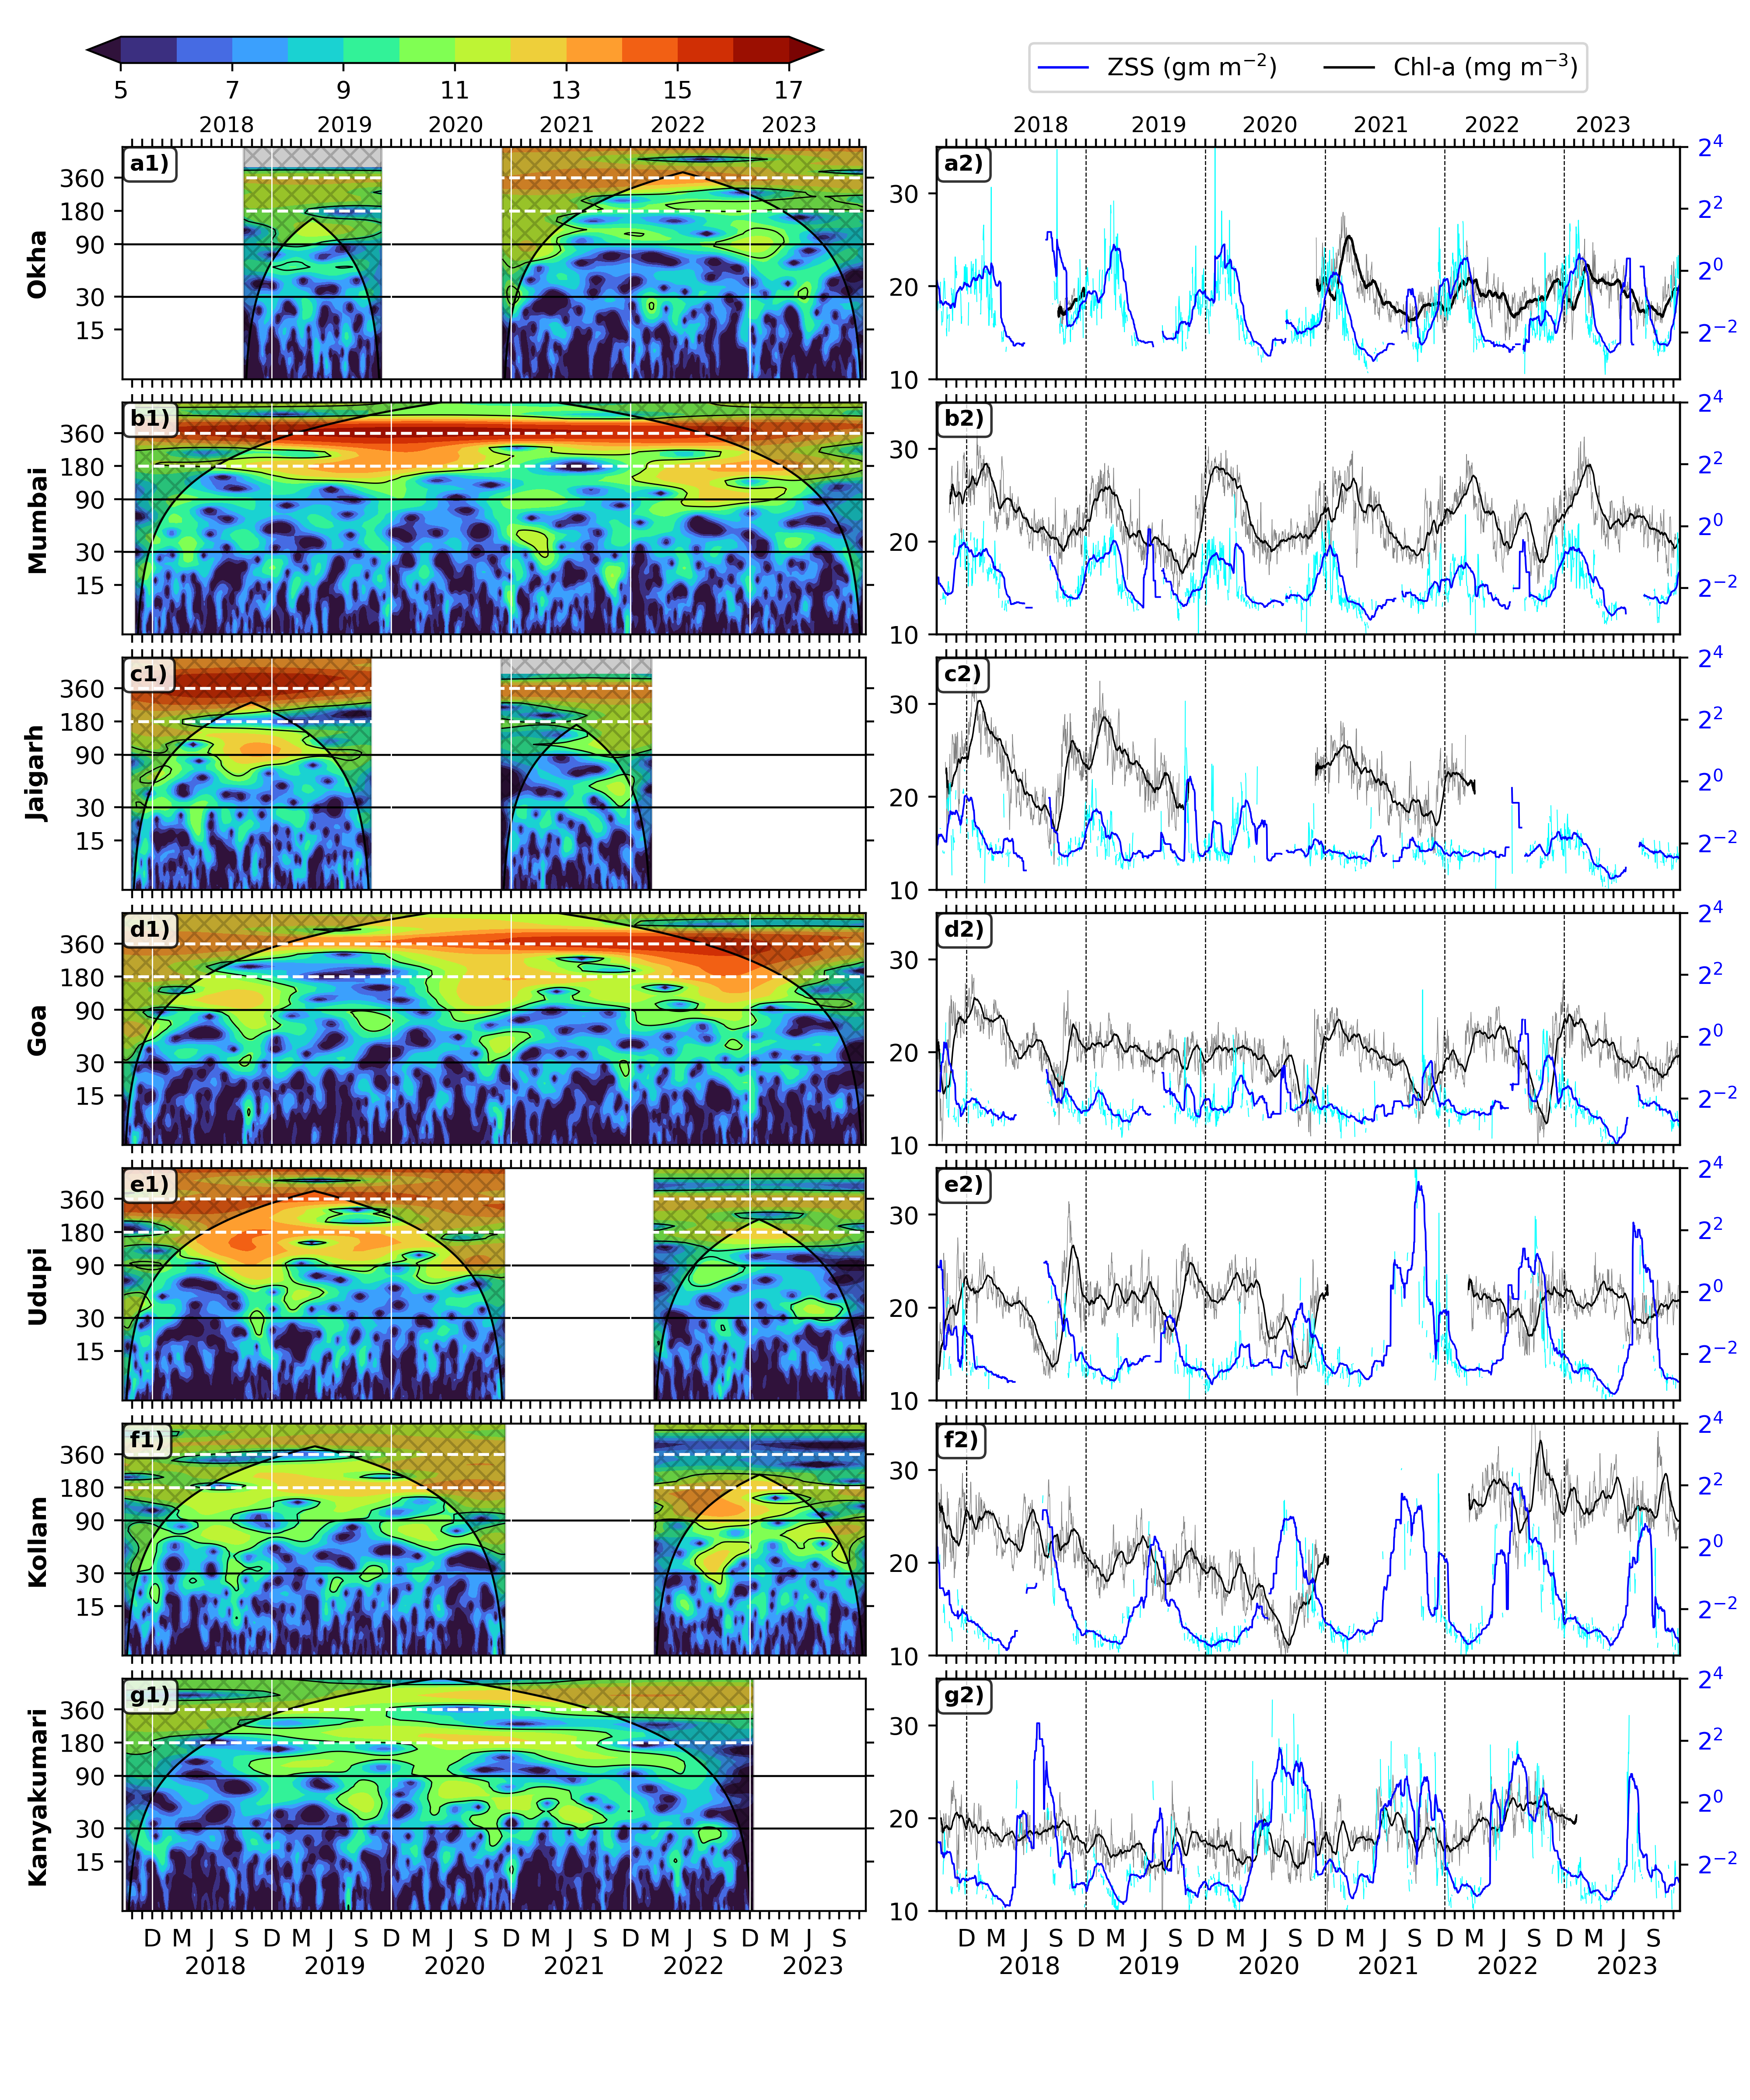
\includegraphics[width=\textwidth]{/media/scilab/disk_ranjan/works/backscatter_wc/figures/west_coast_wavelet_ss_scale.png} 
	\captionsetup{justification=justified,font=footnotesize,skip=0.05\baselineskip,width=\textwidth}
	\caption{Wavelet power spectra (Morlet) of zooplankton standing stock plotted against time as abscissa and period in days as ordinate. The wavelet power is in log$_2$ scale, the 95 \% significance is marked in black contours; The vertical white lines separates years. The right side panel shows the ZSS (24--120 m biomass integral) time series of 30 day rolling mean data (black) overlaid upon daily data (Grey). The 30 day rolling mean data of chlorophyll (solid blue) is plotted over its daily data (cyan).}
	\label{fig:wavess}
\end{figure}

\begin{figure}[htbp]
	\centering
	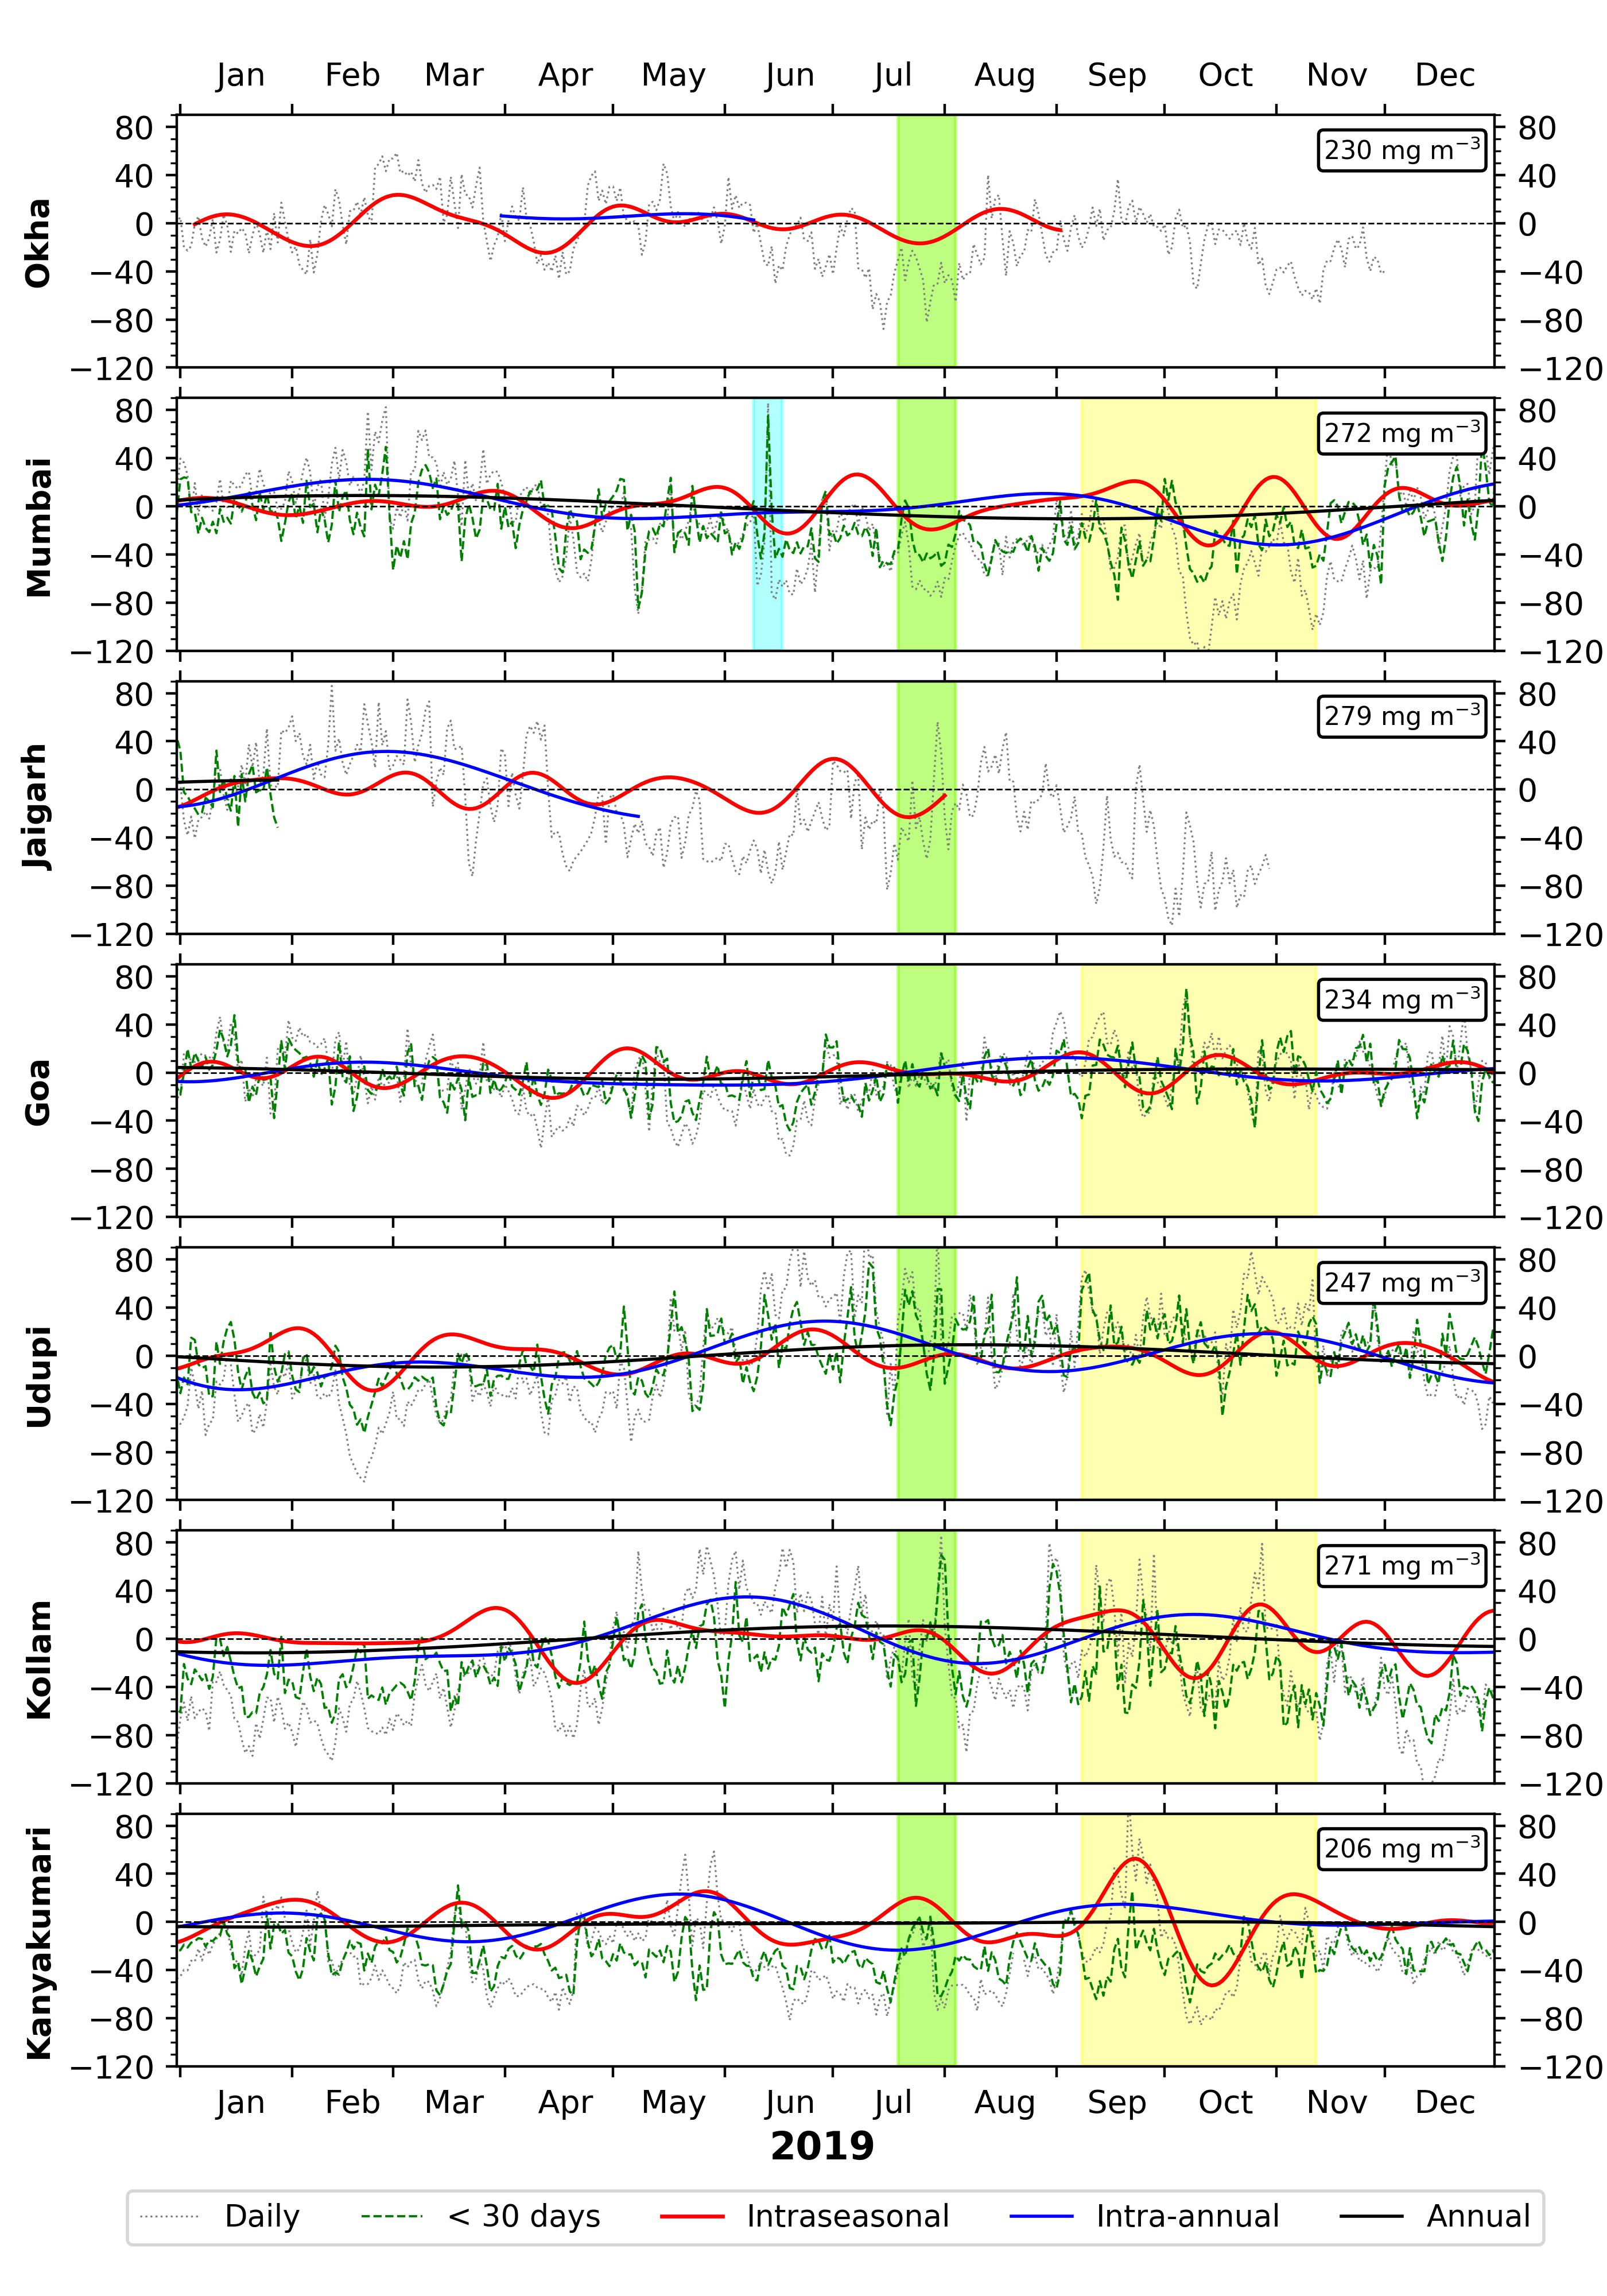
\includegraphics[width=\textwidth]{/media/scilab/disk_ranjan/works/backscatter_wc/figures/biomass_40m_2019_mumbai_goa_kollam.jpeg} 
	\captionsetup{justification=justified,font=footnotesize,skip=0.05\baselineskip,width=\textwidth}
	\caption{Comparison between mean-removed daily biomass time series at 40 m and the distinct components of variability off Mumbai, Goa and Kollam for 2019. The biomass units are mg~m$^{-3}$ and its mean for respective location is shown in top right box.  The cyan curve is sum of all low frequency components above 30 days, i.e, annual, intra-annual and 30 to 90 days intraseasonal variability. Off Mumbai and Kollam, an increase in biomass is noticed from May onward and lasting till late monsoon with weeks of low biomass during August due to contribution from each component of variability.}
	\label{fig:variability}
\end{figure}


\begin{figure}[htbp]
	\centering
	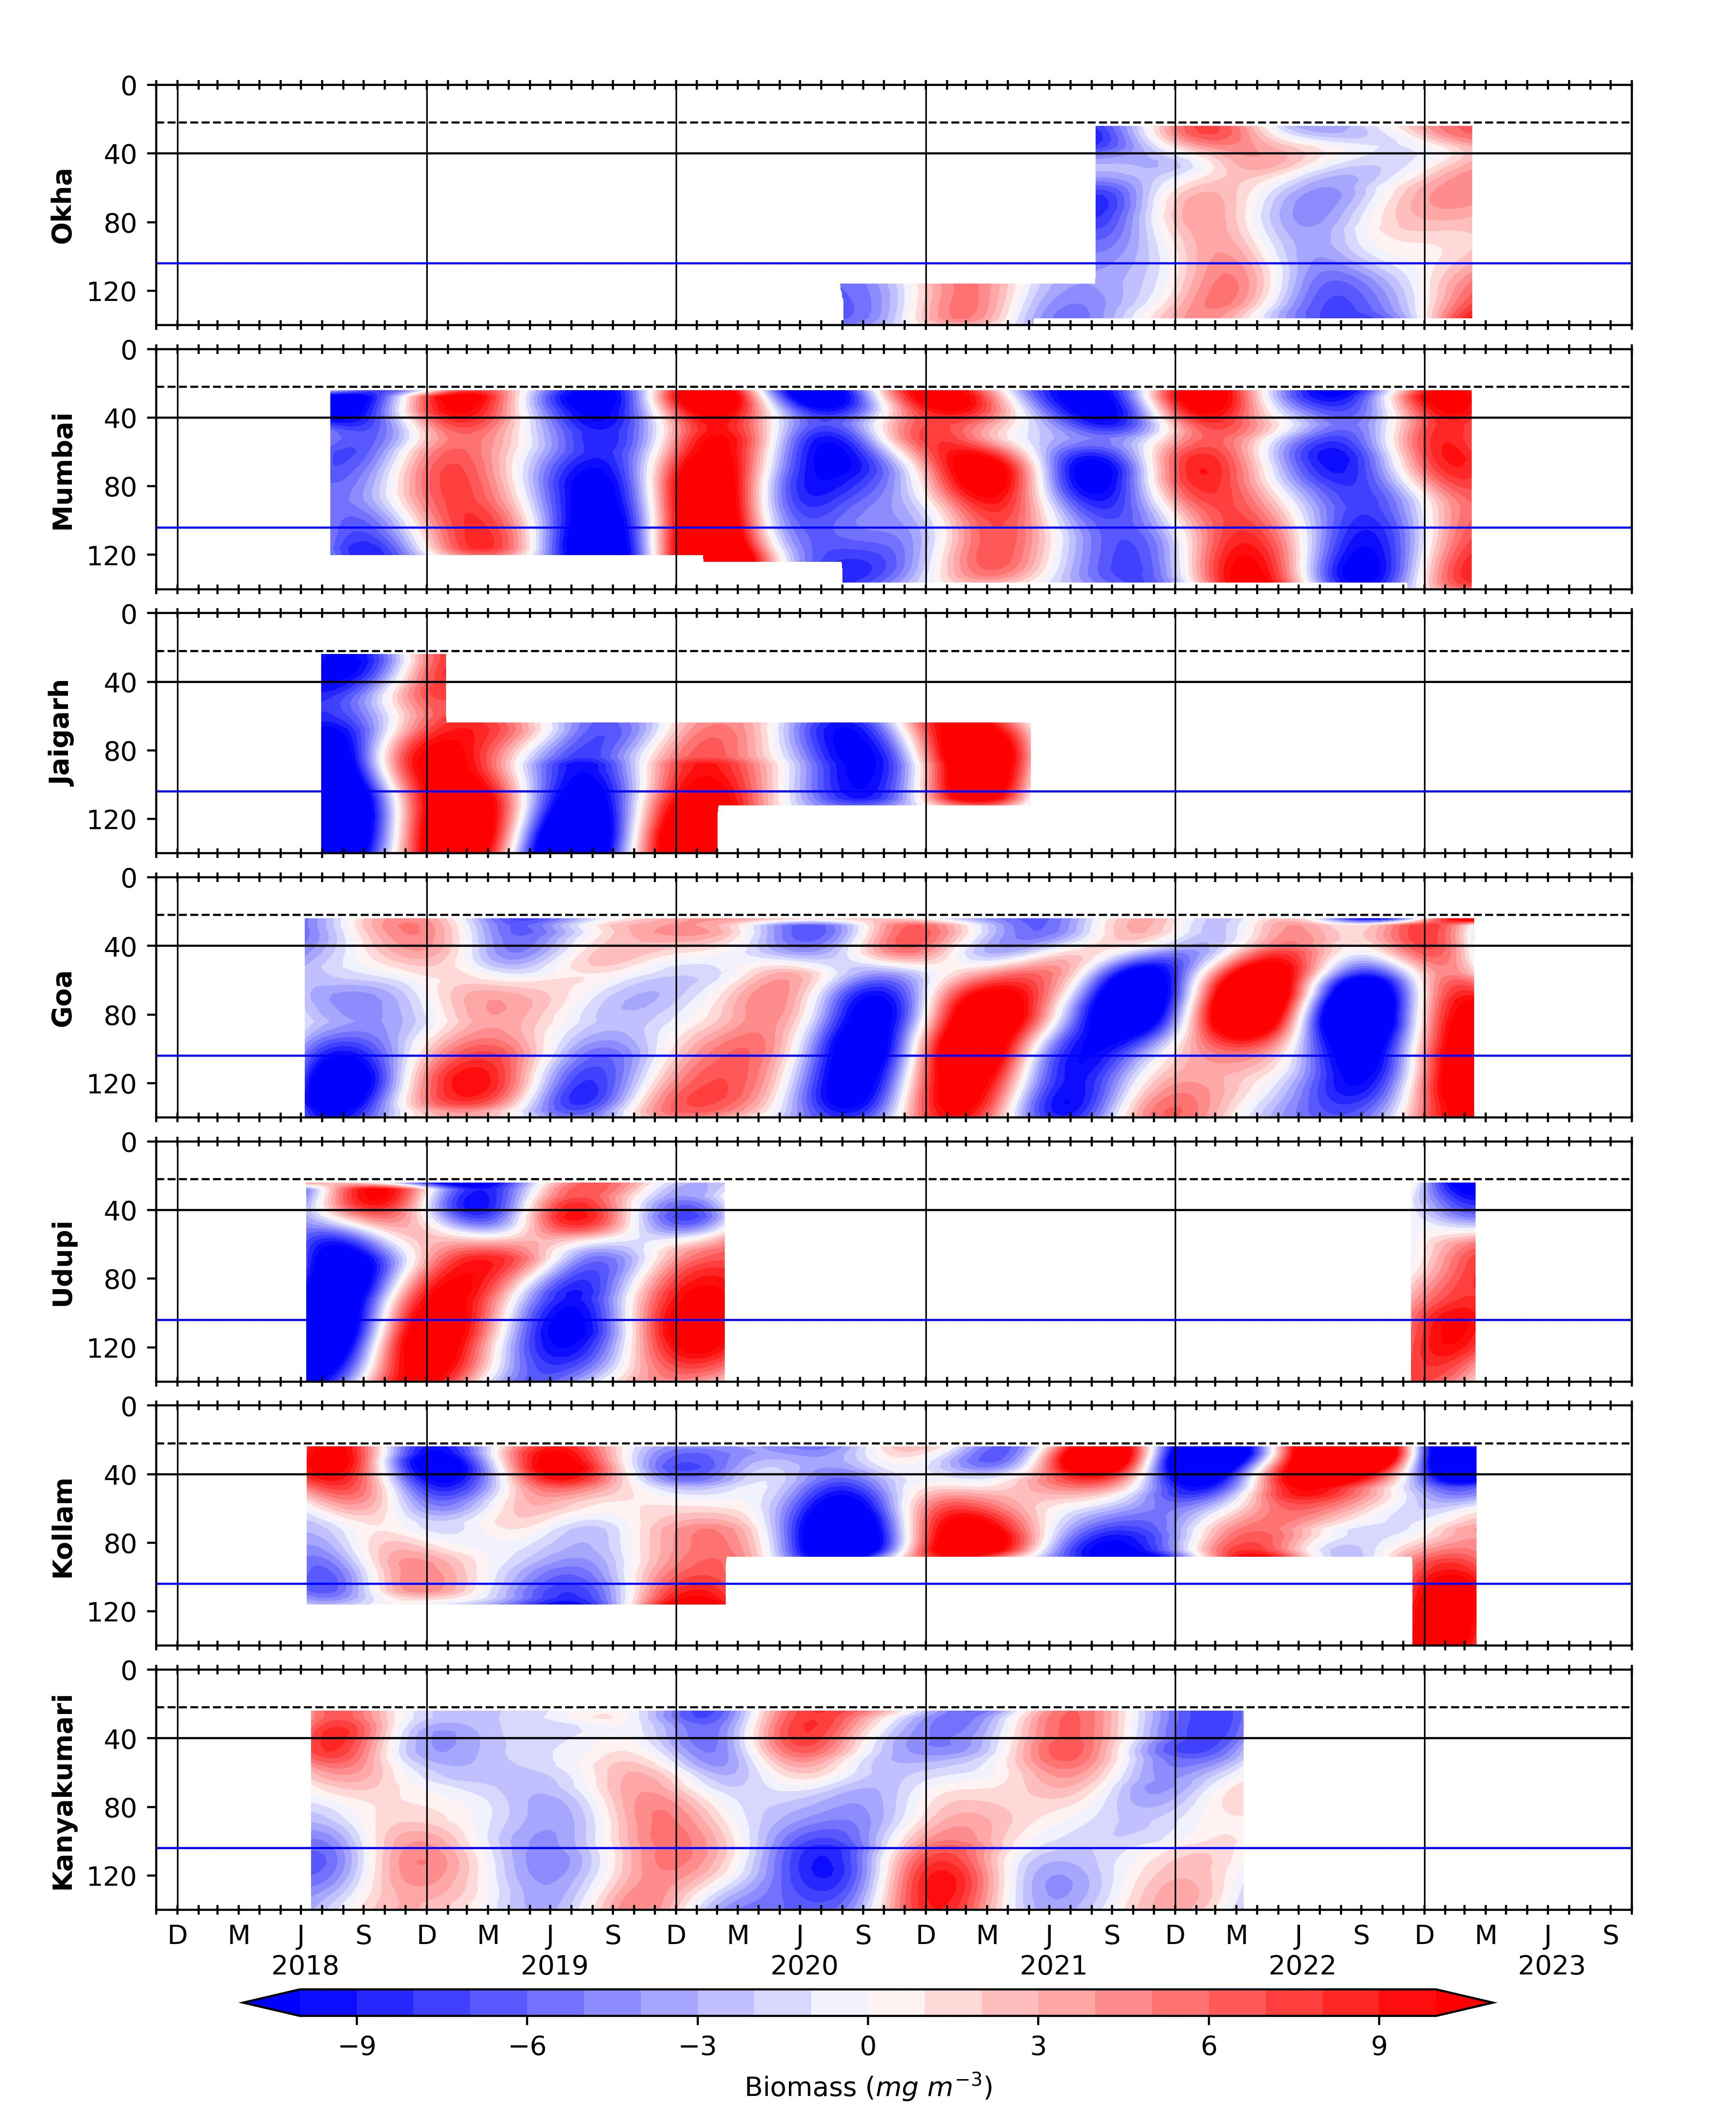
\includegraphics[width=1.05\textwidth]{/media/scilab/disk_ranjan/works/backscatter_wc/figures/annual_300_400_451_1.jpeg} 
	\captionsetup{justification=justified,font=footnotesize,skip=0.05\baselineskip,width=\textwidth}
	\caption{The biomass variation occurring in annual band (300 to 400 days). Owing to the presence of monsoon, there is a variation driven by associated upwelling (downwelling) processes in summer (winter) monsoon. and The horizontal black and blue lines is for 40 and 104 m respectively; vertical black lines separate the years. The dashed line at 22 m marks the top-depth of first bin i.e, 24 m and solid orange curves denotes D215 (D175 off Okha and Kanyakumari)}
	\label{fig:annual}
\end{figure}



\begin{figure}[htbp]
	\centering
	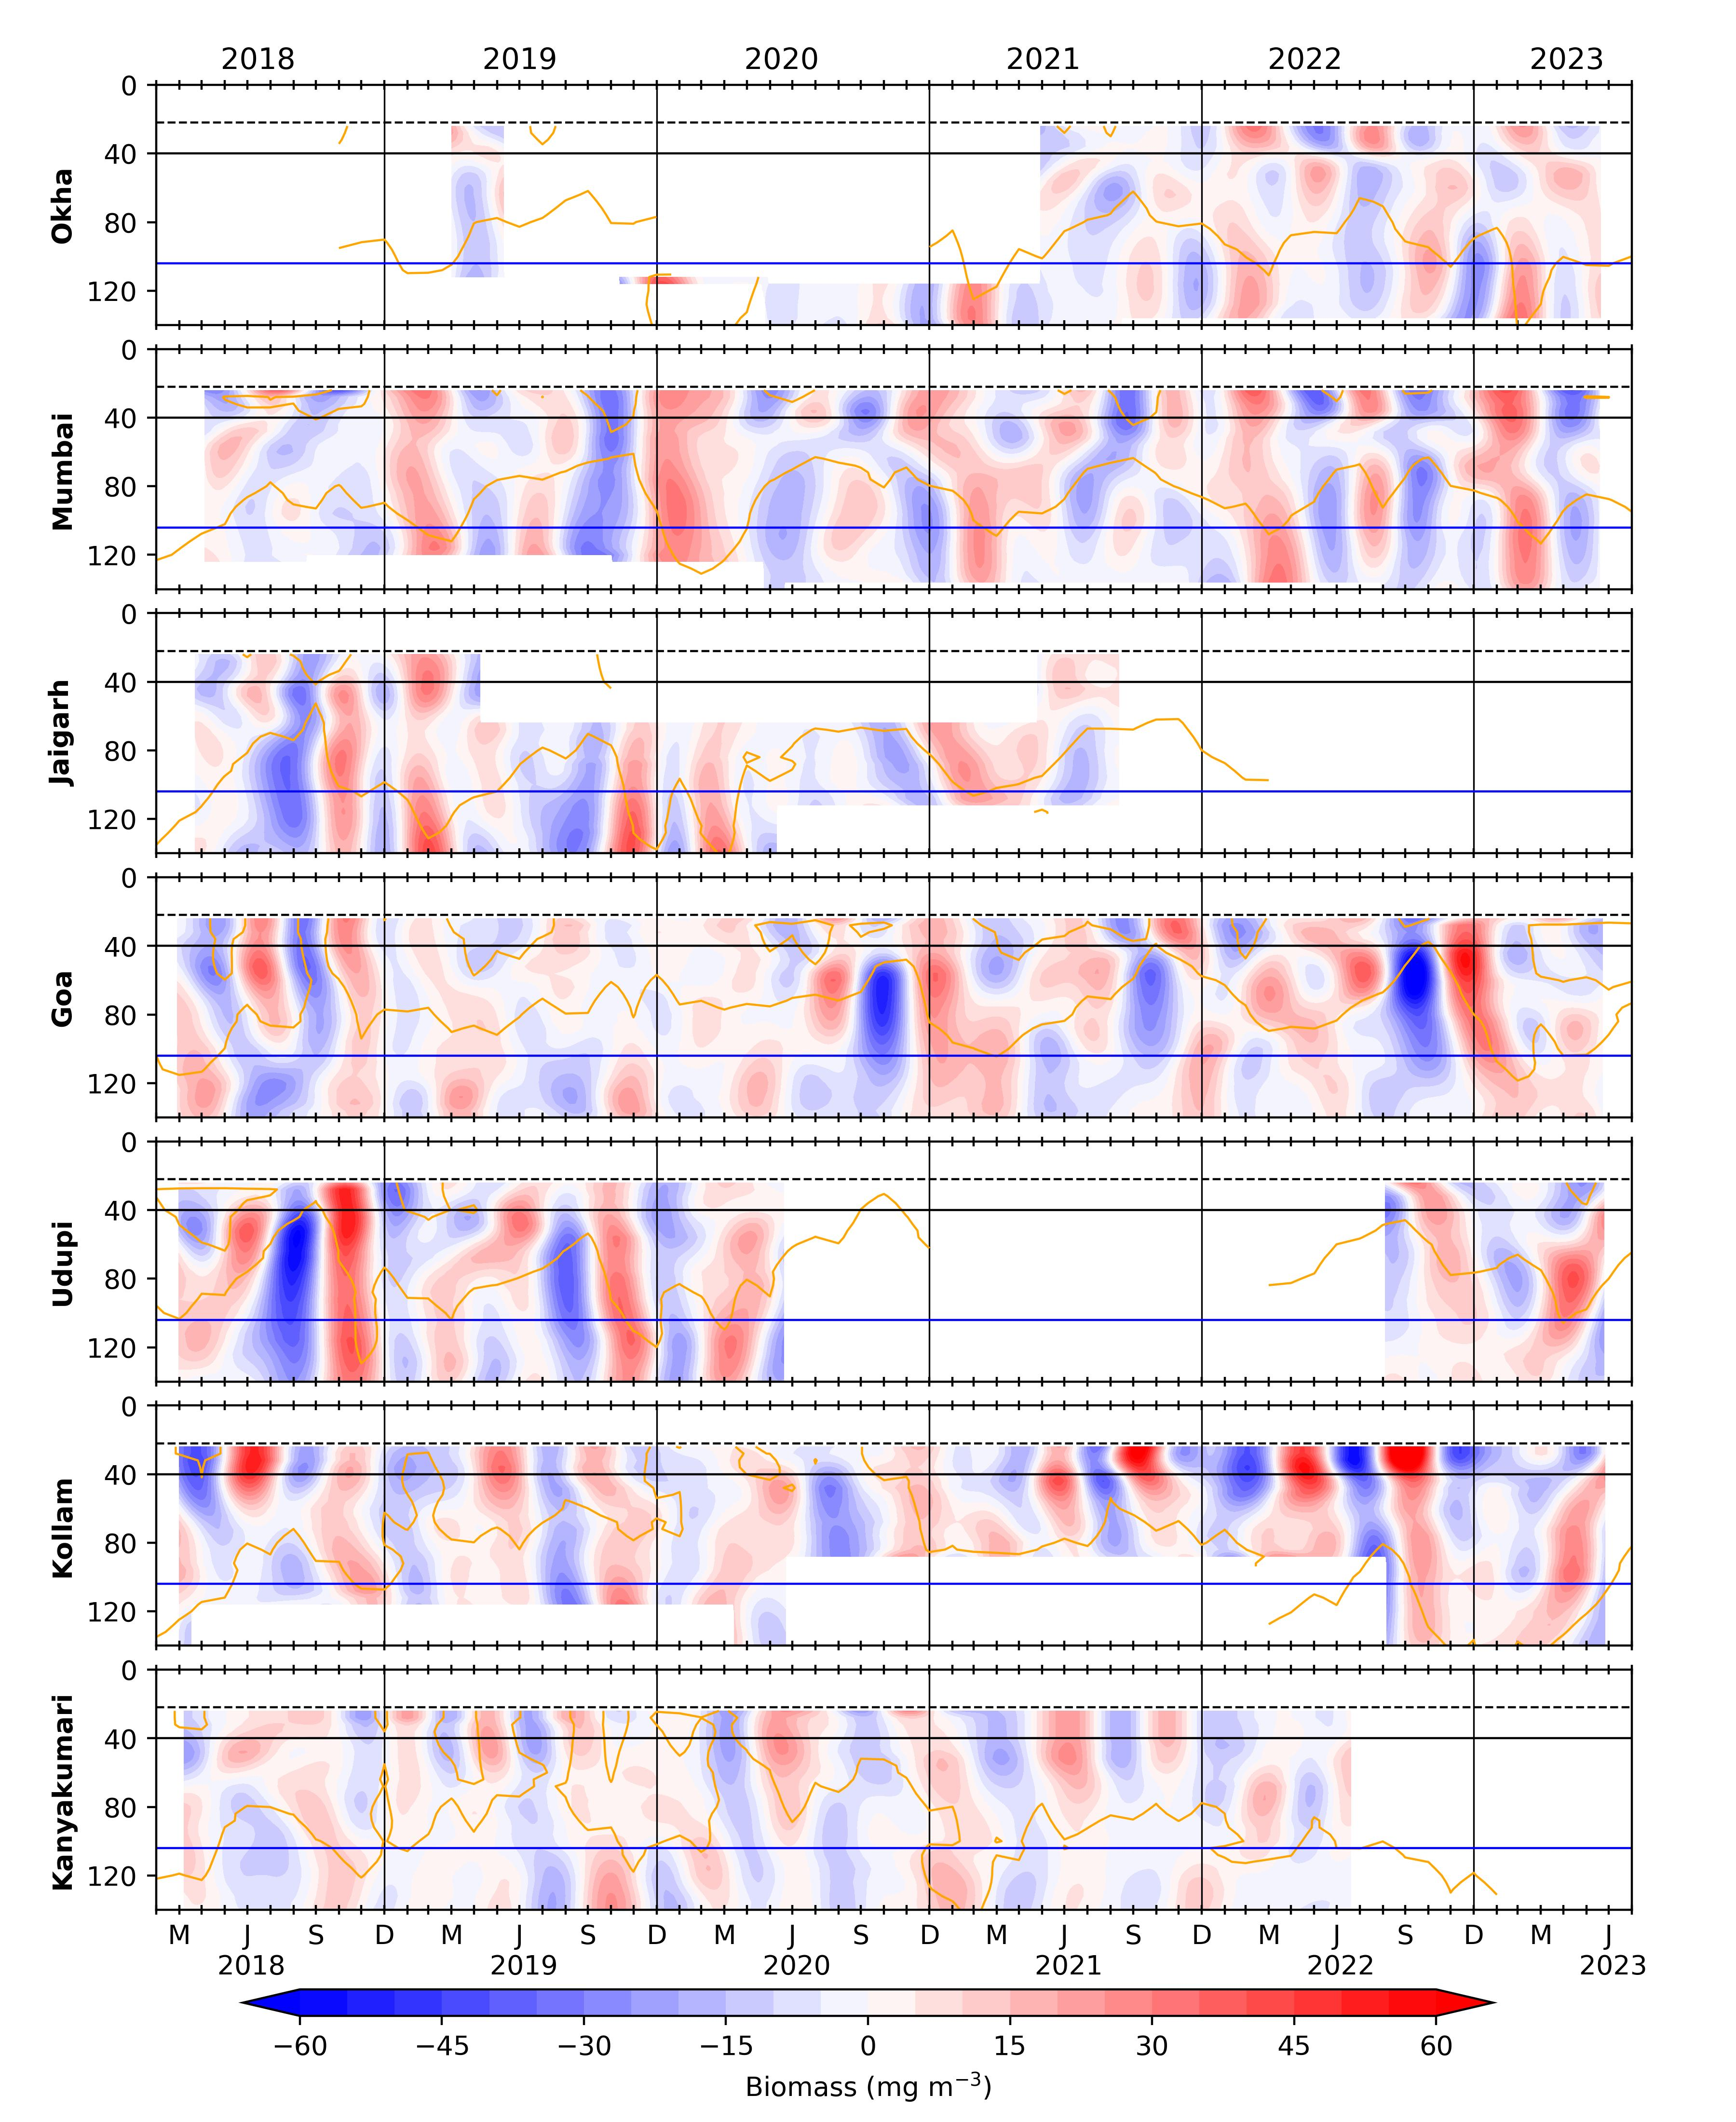
\includegraphics[width=\textwidth]{/media/scilab/disk_ranjan/works/backscatter_wc/figures/intraannual_100_250_351.jpeg} 
	\captionsetup{justification=justified,font=footnotesize,skip=0.05\baselineskip,width=\textwidth}
	\caption{The biomass variation occurring in 100 to 250 days period (between the seasons and within a year record or intra-annual band) is obtained using a band pass filter. The horizontal black and blue lines is for 40 and 104 m respectively; vertical black lines separate the years. The dashed line at 22 m marks the top-depth of first bin i.e, 24 m and solid orange curves denotes D215 (D175 off Okha and Kanyakumari). }
	\label{fig:intraannual}
\end{figure}

\begin{figure}[htbp]
	\centering
	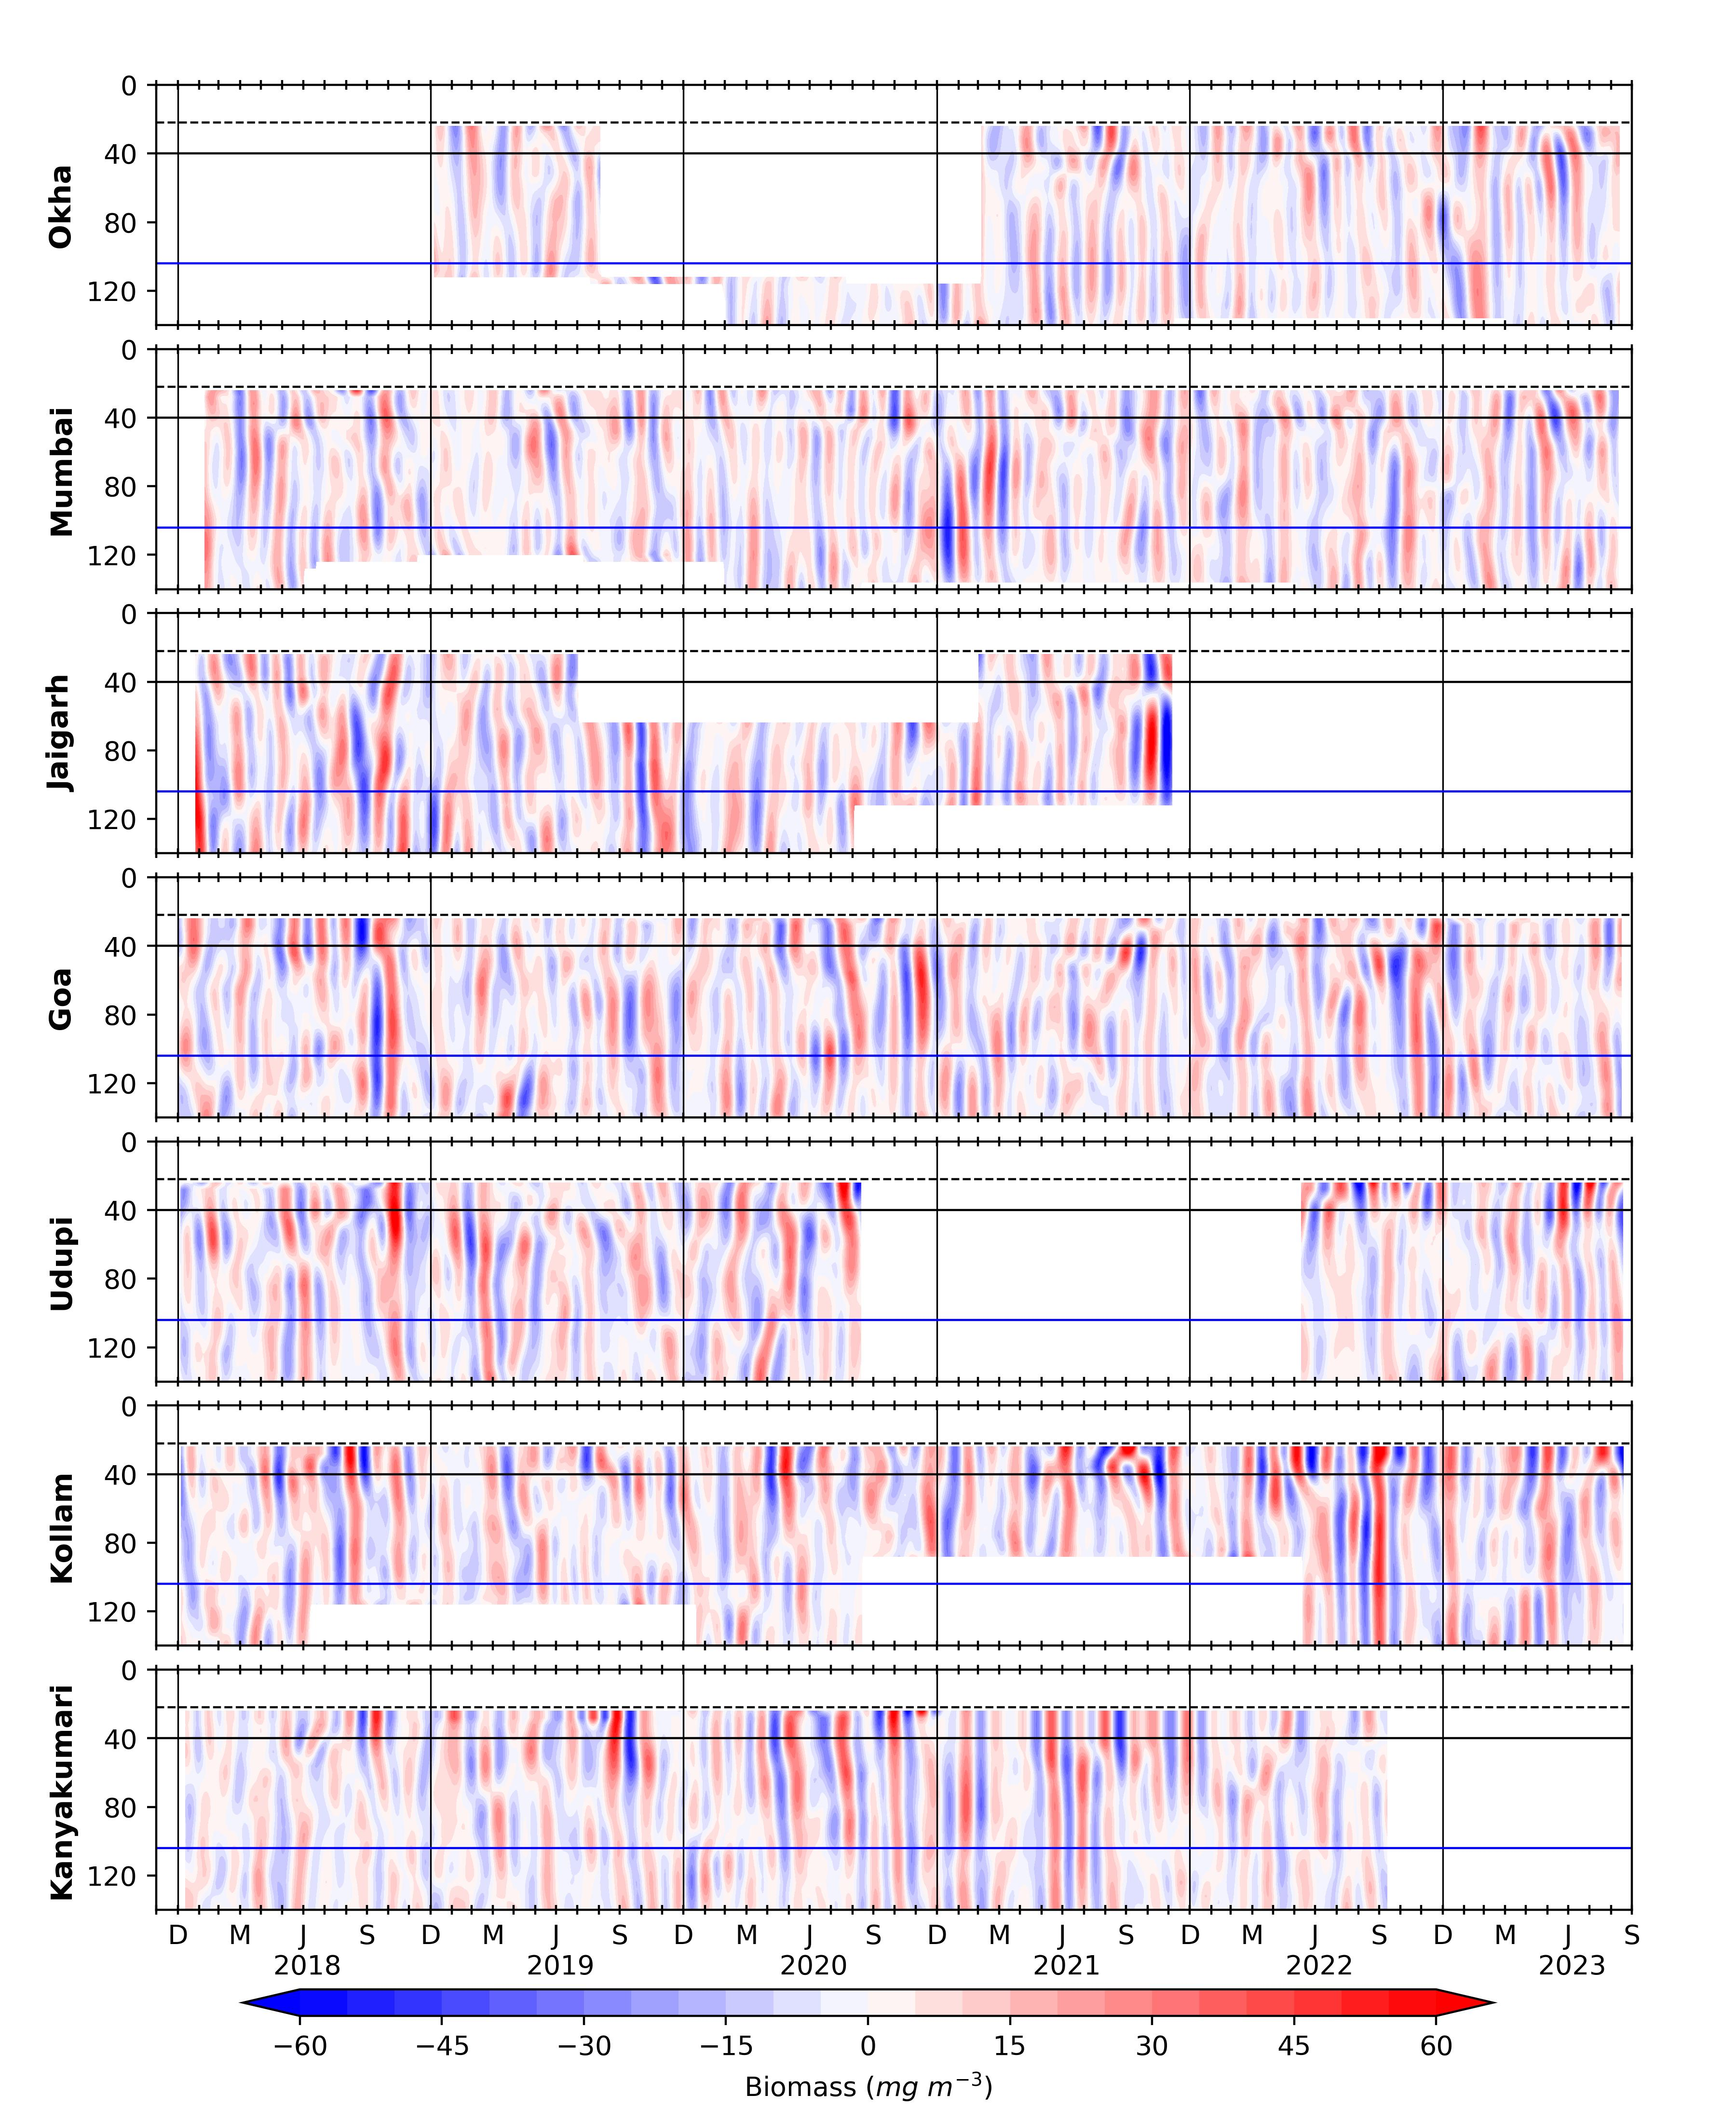
\includegraphics[width=\textwidth]{/media/scilab/disk_ranjan/works/backscatter_wc/figures/intraseasonal_30_90_181.jpeg} 
	\captionsetup{justification=justified,font=footnotesize,skip=0.05\baselineskip,width=\textwidth}
	\caption{Biomass variation found in the Intraseasonal band i.e., 30 to 90 days  period is obtained using a lanczos band pass filter. The horizontal black and blue lines is for 40 and 104 m respectively; vertical black lines separate the years and solid orange curves denotes D215 (D175 off Okha and Kanyakumari). The dashed line at 22 m marks the top-depth of first bin i.e, 24 m. Intraseasonal variability is seen throughout the record, is coherent along the slope and its magnitude is stronger during August to November.}
	\label{fig:intraseasonal}
\end{figure}




\end{document}
